\documentclass[conference]{IEEEtran}

\usepackage[T1]{fontenc}
\usepackage[utf8]{inputenc}
\usepackage{microtype}
\usepackage{booktabs}
\usepackage{array}
\usepackage{graphicx}
\usepackage{flafter}
\usepackage{float}
\usepackage{cite}
\usepackage{url}
\usepackage[hidelinks]{hyperref}
\usepackage{tikz}
\usetikzlibrary{arrows.meta,positioning,shapes.geometric}

\newcommand{\system}{\textsc{Cognalys}}
\newcommand{\researchq}[1]{\textbf{RQ#1}}
\newcommand{\pending}[1]{\textbf{[TODO: #1]}}

\title{Cognalys: A Python Library Complementing RVSec with Evidence-Guided Analysis and Repair}

\author{\IEEEauthorblockN{João Pedro Antonow}
\IEEEauthorblockA{Department of Computer Engineering (CIC)\\
University of Brasilia (UnB)\\
Brasilia, Brazil\\
\texttt{jpantonow@gmail.com}}}

\begin{document}

\maketitle

\begin{abstract}
RVSec reports cryptographic API misuses that an Android application executed,
but not which source change is safe: a fix can depend on stored data, protocol
peers, callers, and application policy. \system, a Python library and
command-line tool, treats each RVSec finding as a claim to check before
repairing it. With repository evidence from the analyzed revision, large
language model stages under deterministic checks decide whether the violation
is real and whether a fix keeps the application's behavior. A confirmed
violation with such a fix, even a rule-only one, becomes a patch applied in an
isolated worktree at the tip of the target branch and built; other findings
end with their reason recorded, or with an issue when their security impact
was confirmed. Nothing is published without explicit human approval.
We report a dated case study of an earlier pipeline version and two
pre-registered evaluations with declared deviations; all results are
descriptive. As of November 18, 2026, of 49 pull requests submitted for RVSec
findings, 21 were incorporated (one only adds a test), 10 were closed, and 18
were open; six of the ten closures questioned the security relevance of the
reported use. When RVSec was rerun on the original and the patched APK, the
reported violation no longer appeared in the patched method for 33 of
the 38 pull requests it could check, and one corrected patch kept
the same key material and only changed how the monitor saw it. On 20 findings, two LLM judges, not
told which arm produced each delivery, compared \system{} with coding agents in
two blocks, counting issue and no-action outcomes as acceptable. Agents given
only the finding and the repository scored close to or above \system{} (0.90
to 0.97, against 0.96) but proposed fewer pull requests and had fewer accepted
(7 to 18, against 28). Agents instructed to follow the same process proposed
more pull requests and had as many or more accepted (28 and 32), but also more
refused (10 and 14, against 3), and scored below \system{} (0.80 and 0.85). Neither the build nor the rerun shows that a patch preserves the
application's behavior.
\end{abstract}

\begin{IEEEkeywords}
cryptographic API misuse, runtime verification, Android, large language
models, program repair, coding agents, open-source contributions, false
positives
\end{IEEEkeywords}

\section{Introduction}
\label{sec:introduction}

Cryptographic API misuses remain common in Java and Android
applications~\cite{nadi2016hoops,torres2023runtime}, and many tools detect
them: static analyzers such as CogniCrypt and CryptoGuard, and dynamic tools
such as CryLogger and RVSec~\cite{krueger2017cognicrypt,krueger2021crysl,
rahaman2019cryptoguard,piccolboni2021crylogger,torres2023runtime}. Detection has
been studied extensively; acting on a report much less. A report says that a
rule was violated, not whether the violation matters in that application or how
to change the program without breaking it. Replacing \texttt{SHA-1} with
\texttt{SHA-256} changes the bytes that storage, synchronization, or a server
expect, and pinning a TLS version removes protocols a peer may still need. The
maintainers who answered our pull requests raised exactly these concerns:
behavior they consider intentional, the compatibility of stored values, and
whether the rule matters in their context (Section~\ref{sec:results}).

RVSec~\cite{torres2023runtime} monitors cryptographic API calls while an
instrumented APK runs and reports each violation at the method that made the
call. Its findings show that the misuse executes, which a static warning does
not, but they refer to a compiled APK rather than to source code: the reported
method may be a Kotlin lambda or coroutine, a name changed by the compiler, or
library code bundled in the app. Turning such a finding into a change a
maintainer can accept takes three further steps: locating the code in the
repository revision the APK was built from, deciding whether the violation is
real and matters there, and producing a patch that keeps the application's
behavior and builds.

Large language models make these steps possible to attempt: they repair code,
sometimes better than earlier repair
systems~\cite{xia2023apr,zhang2023apimisuse}, and coding agents resolve real
repository issues~\cite{jimenez2024swebench}. They also make the steps riskier: generated code can contain security
weaknesses~\cite{pearce2022asleep}, a patch can satisfy its oracle, here the
build, without being correct~\cite{smith2015overfitting}, and a model can be
wrong both about whether a violation matters and about its own patch. A
natural question is whether a general-purpose coding agent is enough, given the
finding and the repository, or given also the same process written as
instructions (Section~\ref{subsec:rq6}). Agents given only the finding and the
repository scored close to \system{} under a measure that counts abstention as
acceptable, but proposed fewer pull requests and had fewer accepted;
agents given the process as instructions proposed more pull requests and had as
many or more accepted, but three to five times as many refused. With the same
model and instructions as \system{} in one arm, the difference is consistent
with executing the process in separate stages, with the decision to act taken
apart from the edit, rather than with the instructions.

This paper presents \system, a Python library and command-line tool for Java
and Kotlin Android applications that checks each API-misuse finding before
acting on it. For every finding it settles, in order, whether the reported
violation actually occurs in the code and whether a fix exists that keeps the
application's behavior. A confirmed violation with such a fix becomes a patch,
whether or not it has security impact. Otherwise the finding ends with its
reason recorded: a false positive, code that already uses the API as documented
(so that any fix would change what it trusts or protects), or a fix that needs
a decision outside the repository; a confirmed violation without a fix becomes
an issue only when its security impact was confirmed. These abstentions are
valid outcomes, not failures. The central design choice is to separate
responsibilities: deterministic components collect evidence, LLM stages
adjudicate, plan, draft, review, and describe the patch under versioned
schemas, and deterministic validators reject unsupported claims, incomplete
plans, known failure shapes, and text that describes edits absent from the
diff. Accepted patches are ported to the tip of the target branch and built
before anyone is asked to publish them, and maintainer responses to earlier
pull requests are read by later analyses. Findings from other detectors in
SARIF or Semgrep JSON format enter the same workflow but are not evaluated
here.

This work makes five contributions:
\begin{itemize}
  \item a Python library and CLI that complement RVSec by connecting each
  runtime finding on an APK to the source revision it came from, to a decision
  on whether it is real, and to a reviewable patch or issue;
  \item a staged design with separate contracts for evidence, adjudication,
  authorized edits, isolated validation, and human review, in which abstention
  and every intermediate decision remain inspectable;
  \item a study of the 49 pull requests and 33 issues submitted to maintainers
  for RVSec findings up to November 18, 2026 (21 pull requests incorporated, 10
  closed, and 18 open), including the reasons maintainers gave for their
  decisions;
  \item a dynamic validation, pre-registered before any new case was built, in
  which RVSec reruns the original and the patched APK of 45 published pull
  requests (33 that met the inclusion criteria and 12 added after their
  results): the reported violation no longer appeared in 33 of the 38 it could
  check; and
  \item a pre-registered comparison on 20 findings with coding agents (Codex
  with two models and Claude Code) in two blocks, given the finding and the
  repository, or also the same process with the port of the patch to the tip of
  the target branch: agents of the first block proposed fewer pull requests and
  had fewer accepted than \system{}; agents of the second block had as many or
  more accepted but more refused (10 and 14, against 3).
\end{itemize}

Section~\ref{sec:background} reviews related work,
Section~\ref{sec:pipeline} describes the pipeline, Section~\ref{sec:settings}
the research questions, a case study of the pipeline as it stood in October
2026, and the two pre-registered evaluations, Section~\ref{sec:results} the
results, and Section~\ref{sec:discussion} implications and threats to
validity; Section~\ref{sec:conclusion} concludes.

\section{Background and Related Work}
\label{sec:background}

\subsection{Cryptographic API Misuses}

An API-use specification describes constraints beyond type checking, such as
calling \texttt{load} before reading a key store, using an adequate digest,
initializing a cipher consistently with its mode, or preventing obsolete
protocol negotiation; some depend on data flow, provider behavior, or runtime
state. Static analyzers such as CogniCrypt
and CryptoGuard check source or bytecode against such rules, and CryLogger
observes values at
runtime~\cite{krueger2017cognicrypt,rahaman2019cryptoguard,piccolboni2021crylogger}.
CrySL, the rule language behind CogniCrypt, combines allowed event sequences,
constraints on values, and predicates that one object passes to
another~\cite{krueger2021crysl}.

RVSec applies runtime verification to the same problem~\cite{torres2023runtime}.
Its cryptographic specifications are JavaMOP monitors translated by hand from
CrySL rules; RVSec weaves them into an APK and exercises the instrumented app
on an emulator with test-generation tools such as Monkey, APE, and DroidBot,
reporting each violation with a code that names the broken constraint and,
when available, the observed and expected values. Runtime and static
techniques expose different sets of misuses and are
complementary~\cite{torres2023runtime}.

Each source of a report carries its own uncertainty. A monitor sees only the
paths the exploration reached, so a misuse behind a login or a setup screen
goes unreported, and different exploration tools reach different code. A rule
may be stricter than the platform's documented behavior: an Android Keystore
algorithm name can be missing from a rule written for desktop providers. Some
reports say that a value was \emph{not observed} to come from an approved
source, such as a key generated outside the monitored run: a limit of tracing,
not a misuse. Static detectors have also shown low precision and
recall~\cite{amann2019evaluation}. A finding is thus evidence, not proof that a
particular edit is correct.
\system{} turns three of these uncertainties into questions it answers before
any edit: it maps the reported method back to source, checks the rule against
the platform's documented behavior, and lets the adjudication conclude that a
tracing limit is not a misuse (Section~\ref{sec:pipeline}). Coverage remains
the detector's limit.

\subsection{Automated Repair and Coding Agents}
\label{subsec:apr}

Automated program repair (APR) produces candidate patches for a reported
defect and keeps those that an oracle, usually the project's tests,
accepts~\cite{legoues2019apr}; a patch can satisfy that oracle without fixing
the defect, a problem known as patch
overfitting~\cite{smith2015overfitting}. \system{} has no test that encodes
the misuse: a patch is accepted when it passes the deterministic checks and
the behavior review, applies, and builds, and none of these observes whether
the violation is gone. The evaluation therefore asks the detector again,
rerunning RVSec on the original and the patched APK of published pull requests
(Section~\ref{subsec:dynval}). That check is also indirect, since a report
disappears too when the exploration no longer reaches the patched code; it
also shows whether patches that change the code but not what the monitor
observes, which the behavior review should reject, were still published.

LLM-based repair~\cite{xia2023apr,zhang2023apimisuse} takes the reported
defect as given, the premise our maintainers questioned; \system{} therefore
decides whether a finding is real and has a behavior-preserving fix before it
generates any edit.

Coding agents run a model in a loop with tools, reading and editing files and
running commands until the model decides the task is
done~\cite{yang2024sweagent}. SWE-bench accepts a patch for a real GitHub issue
when tests taken from the pull request that resolved it
pass~\cite{jimenez2024swebench}, and SWE-agent showed that the interface
through which an agent views and edits a repository changes how many issues it
resolves~\cite{yang2024sweagent}. The Codex CLI~\cite{openai2026codex} and
Claude Code~\cite{anthropic2026claudecode} run the same loop on a developer's
machine. Their oracle defines what ``resolved'' means, so a patch that passes
the issue's tests can still overfit them. An agent also follows a process only
as far as it follows its instructions, whereas \system{} runs each stage in code and checks its output
before the next one starts. The comparison of Section~\ref{subsec:protocol}
gives coding agents \system{}'s process as instructions, including the port to
the branch tip, so it measures the difference between a process that is
instructed and one that is enforced.

\subsection{Tool-Generated Contributions to Open Source}
\label{subsec:bots}

In a study of popular GitHub projects, about a quarter used bots, and
maintainers judged them useful but limited~\cite{wessel2018bots}. Automated
pull requests that upgrade out-of-date dependencies led projects to upgrade
more often, but many were left unmerged, with developers citing the risk of
breaking changes and the effort of understanding the
change~\cite{mirhosseini2017autopr}. Pull requests opened by bots are merged
less often and wait longer for a response than those opened by
people~\cite{wyrich2021botprs}. A dependency update can be checked against a
release; a fix for an API misuse changes the project's own code, and whether it
is wanted depends on what that code protects. Every pull request and issue in
this study was approved by the author before it was opened;
Section~\ref{subsec:form} shows how maintainers responded to the form of the
first submissions and how the text changed.

\subsection{LLMs as Judges}
\label{subsec:judges-bg}

On chat-assistant questions, strong LLM judges agreed with human raters about
as often as humans agreed with each other, but favored answers by position,
longer answers, and their own outputs~\cite{zheng2023judge}. The order in which
candidates are shown can change a verdict~\cite{wang2024fair}, and LLM
evaluators recognize and favor their own
generations~\cite{panickssery2024selfpref}. On software engineering artifacts,
LLM ratings approach human agreement on some annotation tasks but not others,
and agreement between models signals when they can be
trusted~\cite{ahmed2025annotation}. The comparison of
Section~\ref{subsec:protocol} uses two judges from different providers and
addresses these biases: cards are scored in random order; one reading shows
only the patch, without its title and description; scores are reported per
judge, with the difference between what a judge gives its own model family and
what the other judge gives it; and a probe asks a judge to name the arm behind
a card. A residual risk remains: when the judges disagree, the final score is
the principal judge's, which belongs to the same family as one agent arm, while
the other judge is the model of another arm. The reference answers were
revised twice after results had been seen; every version is kept with the
data.

\subsection{Positioning of This Work}

Table~\ref{tab:related} relates \system{} to prior work. Detectors, RVSec among
them, end with a report, which \system{} treats as a claim to check against the
source revision, without assuming security impact; repair tools and coding
agents end with a patch that tests or a build accept, whereas \system{} can end
with a reasoned decision not to change the code. The closest work, a preprint
by Zhang et al., evaluates pretrained language models on API-misuse
repair~\cite{zhang2023apimisuse}. The present study differs in four ways: it
starts from runtime findings on APKs and repairs their source revision; it
counts a reasoned abstention as a valid outcome; it records every intermediate
decision for inspection; and its patches went to real maintainers and were
checked again by RVSec, rather than scored only on a benchmark.

\begin{table*}[t]
\centering
\caption{Relationship to representative prior work.}
\label{tab:related}
\footnotesize
\begin{tabular}{p{2.9cm}p{3.1cm}p{3.4cm}p{6.0cm}}
\toprule
Work & Primary input & Main outcome & Relation to \system \\
\midrule
CrySL and CogniCrypt~\cite{krueger2017cognicrypt,krueger2021crysl} &
Java programs and declarative crypto rules & Static misuse reports; code
templates for common tasks & CrySL rules are the origin of RVSec's
specifications; \system{} takes misuse reports as input and decides whether
and how to change the code. \\
CryptoGuard~\cite{rahaman2019cryptoguard} & Java and Android programs &
High-precision static warnings & Prunes false positives by program analysis
but proposes no repair. \\
CryLogger and RVSec~\cite{piccolboni2021crylogger,
torres2023runtime} & Executions and runtime specifications & Concrete misuse
observations & Provide dynamic evidence but not a conservative source-repair
workflow. \\
LLM-based APR~\cite{xia2023apr,zhang2023apimisuse} &
Faulty code and its context & Candidate patches on benchmarks & Measures patch
generation; \system{} adds abstention, edits authorized per file and symbol, a
build in the real project, and human approval before publication. \\
SWE-bench and SWE-agent~\cite{jimenez2024swebench,yang2024sweagent} &
Repository and issue text & Patch accepted by the issue's tests & Same
repository-level setting; \system{} starts from analyzer evidence and checks a
patch with a build, a static rule when one exists, and a model review of its
behavior; our evaluation also reruns RVSec on the patched app. \\
Codex CLI, Claude Code~\cite{openai2026codex,anthropic2026claudecode}
& Repository and a task in natural language & Edits made in an agent loop &
Baselines of our comparison, given \system{}'s process as instructions. \\
Pull requests from bots and tools~\cite{mirhosseini2017autopr,wessel2018bots,
wyrich2021botprs} & Outdated dependencies, project events & Pull requests for
maintainers & Their changes are checked by an existing oracle, such as a
release; \system{}'s changes alter security-relevant code, and each is
approved by a person before it is sent. \\
\bottomrule
\end{tabular}
\end{table*}

\section{The \system{} Pipeline}
\label{sec:pipeline}
\label{subsec:library}

\system{} is a Python library and command-line tool that turns each finding
reported by a detector into a reviewed outcome: a repair proposal, an issue
for the maintainers, or a documented decision not to propose anything
(Figure~\ref{fig:pipeline}). Each stage writes its results to the run
directory instead of passing an opaque conversation to the next one, so every
decision can be traced back to the evidence it used.

\begin{figure*}[t]
\centering
\resizebox{\textwidth}{!}{%
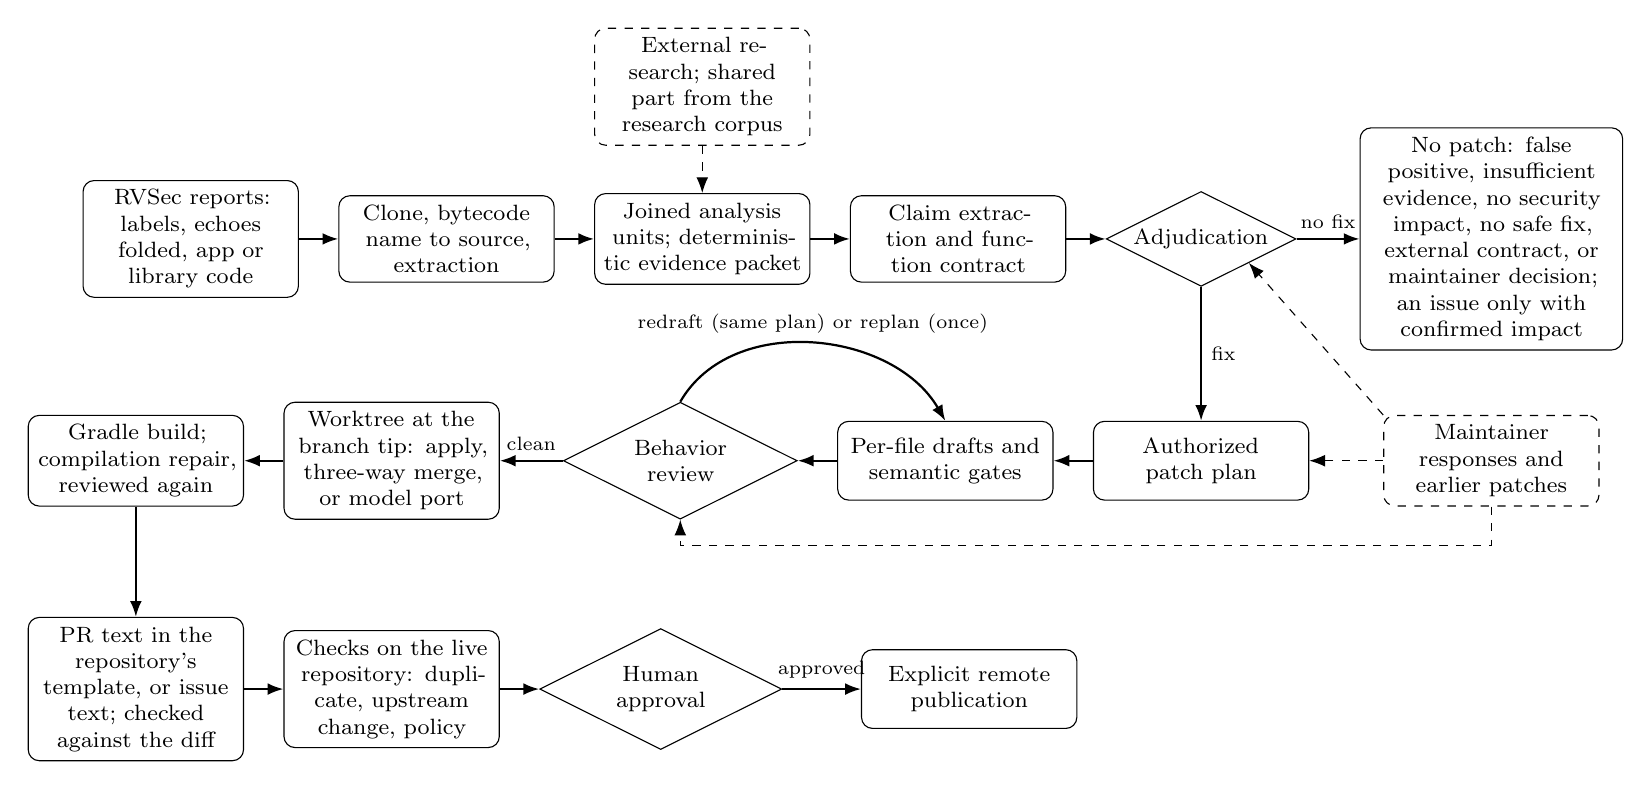
\begin{tikzpicture}[
  node distance=5mm and 5mm,
  box/.style={draw,rounded corners,align=center,minimum height=10mm,
              text width=2.5cm,font=\footnotesize},
  aux/.style={draw,dashed,rounded corners,align=center,minimum height=8mm,
              text width=2.5cm,font=\footnotesize},
  gate/.style={draw,diamond,aspect=2,align=center,font=\footnotesize,
               inner sep=1pt,text width=1.7cm},
  flow/.style={-{Latex[length=2mm]},thick},
  feed/.style={-{Latex[length=2mm]},dashed},
  lbl/.style={font=\scriptsize}
]
\node[box] (csv) {RVSec reports: labels, echoes folded, app or library code};
\node[box,right=of csv] (extract) {Clone, bytecode name to source, extraction};
\node[box,right=of extract] (packet) {Joined analysis units; deterministic evidence packet};
\node[box,right=of packet] (claims) {Claim extraction and function contract};
\node[gate,right=of claims] (adj) {Adjudication};
\node[box,right=8mm of adj,text width=3.1cm] (abstain) {No patch: false positive, insufficient evidence, no security impact, no safe fix, external contract, or maintainer decision; an issue only with confirmed impact};
\draw[flow] (csv)--(extract);
\draw[flow] (extract)--(packet);
\draw[flow] (packet)--(claims);
\draw[flow] (claims)--(adj);
\draw[flow] (adj)--node[above,lbl]{no fix}(abstain);
\node[aux,above=6mm of packet] (corpus) {External research; shared part from the research corpus};
\draw[feed] (corpus)--(packet);
\node[box,below=17mm of adj] (plan) {Authorized patch plan};
\node[box,left=of plan] (gen) {Per-file drafts and semantic gates};
\node[gate,left=of gen] (review) {Behavior review};
\node[box,left=8mm of review] (apply) {Worktree at the branch tip: apply, three-way merge, or model port};
\node[box,left=of apply] (repair) {Gradle build; compilation repair, reviewed again};
\draw[flow] (adj)--node[right,lbl]{fix}(plan);
\draw[flow] (plan)--(gen);
\draw[flow] (gen)--(review);
\draw[flow] (review)--node[above,lbl]{clean}(apply);
\draw[flow] (apply)--(repair);
\draw[flow] (review.north) to[out=60,in=120] node[above,lbl]{redraft (same plan) or replan (once)}(gen.north);
\node[aux] (memory) at (abstain |- plan) {Maintainer responses and earlier patches};
\draw[feed] (memory)--(plan);
\draw[feed] (memory.north west)--(adj.south east);
\draw[feed] (memory.south) -- ++(0,-5mm) -| (review.south);
\node[box,below=14mm of repair] (text) {PR text in the repository's template, or issue text; checked against the diff};
\node[box,right=of text] (checks) {Checks on the live repository: duplicate, upstream change, policy};
\node[gate,right=of checks] (publish) {Human approval};
\node[box,right=10mm of publish] (public) {Explicit remote publication};
\draw[flow] (repair)--(text);
\draw[flow] (text)--(checks);
\draw[flow] (checks)--(publish);
\draw[flow] (publish)--node[above,lbl]{approved}(public);
\end{tikzpicture}
}
\caption{Workflow exposed by the Python library and CLI. Dashed inputs inform
decisions but cannot authorize an edit: only repository evidence and explicit
policy can.}
\label{fig:pipeline}
\end{figure*}

\subsection{From an RVSec Report to Source}

A data table in \system{} states what each RVSec label asserts: a value the
check does not admit, calls out of the rule's order, an origin the monitor did
not observe, an observed origin it does not admit, or an echo of a report about
the object's producer. An echo is folded into the findings of the method it
repeats unless its origin lies elsewhere. A finding is marked as application or
library code from the app's own packages (the namespaces of every module in the
repository); reports on obfuscated class names are set aside. When \system{}
starts the RVSec run, the APK is built without minification where the F-Droid
recipe allows, so runtime locations map back to source. The runtime observation
stays in the evidence, and its label bounds what the report establishes: an
unobserved origin states what the monitor saw, not what the object is---an IV
generated by the cipher provider is random although the monitor cannot trace
it.

The workflow clones the repository, records the documented base branch, reads
its guidance files, and maps the bytecode method to a source declaration.
Kotlin value-class mangling and compiler suffixes are removed; a lambda or
coroutine body that names no source function maps to the one function of its
outer class that uses the governed API or, failing that, to the one function it
calls in the same Gradle module that does; a method missing from the resolved
file is sought in the package's other files; and in Kotlin Multiplatform the
Android source set is preferred to desktop or iOS code the APK never contains.
An ambiguous match stays unresolved instead of guessed. Conservative
Tree-sitter indexes of Java and Kotlin supply the exact method, class context,
callers, overrides, references, value consumers, tests, dependencies, minimum
SDK, and Gradle configuration; relations that need a full JVM classpath stay
explicitly ambiguous. Target source is never truncated; a budget limits
auxiliary context and records every exclusion.

Findings in one piece of code form one unit with one patch: same class and
file, and either one method calls the other, one method violates two rules, or
one rule and message recur along one object's lifecycle. Findings of one
specification in different classes of a module also join when one method
stores a value the other reads back, such as an IV written at encryption and
read at decryption. Separate drafts for such findings rewrote the same code in
incompatible ways. A unit ends before any model call when each finding already
has a pull request of ours that is open or was merged after the analyzed
revision, or when the reported file is not on the target branch.

\subsection{Specifications and external research}

Each rule family has a JSON specification of governed types, events, detector
and runtime semantics, known false-positive shapes, and evidence requirements,
separating what a detector message asserts from what would establish runtime
harm (a literal \texttt{TLS} warning does not reveal the negotiated protocol).
Specifications are written by a model from the rule and official documentation
and audited deterministically against the cited rule, so a dropped event or an
added value is visible before it shapes an analysis.

Optional external research is a separate model call restricted to official and
primary sources; web or repository content is untrusted data that cannot
instruct the pipeline, choose files, or authorize publication. Its shared part,
about the API and rule, is kept in a research corpus and reused for up to 90
days only by a byte-identical request (same prompts, schema, model, effort,
output limit, and search tool); the case part is always researched. The case
study and published pull requests predate the corpus; the comparison's runs
record the state they started from (Section~\ref{subsec:frozen}).

\subsection{Evidence packet and LLM contracts}

Python builds an evidence packet per unit; each item has an identifier,
provenance, trust level, completeness state, and hash. Runtime observations and
exact source outrank semantic relations, official documentation, primary
research, secondary sources, and model inference. Absence is
\texttt{not\_found\_in\_examined\_scope}, \texttt{confirmed\_absent}, or
\texttt{unknown\_due\_to\_}\allowbreak\texttt{incomplete\_scope}, never used
interchangeably. Six model contracts follow:
(1)~\emph{evidence extraction} classifies claims as confirmed, inferred,
hypothesis, or unknown, citing evidence IDs, and states the code's function
contract---its purpose, its counterpart (a third-party service, a peer the user
operates, or the same app or device), and whether that counterpart depends on
the reported behavior, quoting repository code outside the reported method
verbatim; (2)~\emph{adjudication} decides cause, violation, runtime security
impact, compatibility, scope, generation and publication blockers, and the
disposition; (3)~\emph{planning} authorizes every file, symbol, edit kind,
invariant, and test, without code; (4)~\emph{generation} returns exact
per-file replacements; (5)~\emph{behavior review} reads the finished patch
against the whole file and the plan's invariants and forbidden changes, and
answers every adjudication concern; (6)~\emph{proposal text} describes the
final diff. When extraction names missing evidence or adjudication abstains for
lack of it, Python fetches it and both run once more, keeping the new answer
only if it validates. Narrower schema-checked stages handle research,
compilation repair, and the port to the branch tip.

Adjudication chooses among fifteen decisions in five groups: repairs applied
and built without further review (single- or multi-file fix, internal digest
migration, dependency fix or replacement); repairs a person must read before
application (multi-file fix, backend or multi-repository migration); decisions
awaiting explicit policy; confirmed violations needing no change here
(non-security digest use, no security impact, or an external digest contract
no client-side change can meet); and \texttt{NO\_SAFE\_FIX}. A review-only
decision may allow local application for validation while blocking
publication. Hashes of prompt, schema, policy, specification, context builder,
and resolver make runs comparable.

\subsection{Deterministic safeguards and residual trust}

Deterministic checks guard each transition, because structured output does not
make a conclusion true. A confirmed claim citing an unknown evidence ID is
rejected; a supported adjudication needs a confirmed cause and detector
violation; a plan must cover every file the scope requires, and each generated
file must match a plan entry. Each replacement must occur exactly once in the
base source; unauthorized paths, unsupported edit categories, incomplete
coordinated edits, and cross-file symbol inconsistencies are rejected; build,
dependency, public-interface, and new-file edits need explicit categories.
Semantic gates reject known failure shapes: changing a stored, transmitted, or
constant-compared value without keeping the old form for existing data; leaving
a reader of a changed stored value unchanged; removing a user setting's
behavior or ciphertext the app ships; replacing a protocol-mandated algorithm;
or leaving the reported value untouched. Each rejection returns to the
generator with the reason; when no in-app change can satisfy it (ciphertext
under a shipped key, a weaker behavior the user opted into), the finding goes
to the maintainers by the routing below. A rename must update every reference
in the same patch, or is regenerated with the failure explained; whether to
authorize it is a note in the pull request, not a block.

Trust remains: the index is not a complete JVM analysis, a resolved call may
depend on dispatch, reflection, or generated code, and documentation describes
an API contract, not the deployed provider. Unresolved assumptions stay
visible as \emph{review assumptions} for a maintainer or test, distinct from
\emph{generation blockers} (code would be unsupported) and \emph{publication
blockers} (buildable locally, not presented as ready).

\subsection{Behavior review and routing}

A regression needs a concrete scenario reachable through the application's own
code. Removing something deprecated or insecure offered to or accepted from a
peer is hardening unless evidence shows who depends on it: the function
contract, an option in the code, other code handling that peer, or the
maintainers. The review attributes each regression to the plan (no draft
following it can avoid the scenario) or to the draft. A draft's slip is
redrafted on the same plan with the scenario as feedback, regenerating tests
whose production file that feedback changes. After the plan's last draft, or
two consecutive plan-caused regressions, the unit is replanned with the
scenarios as constraints---at most once for any reason; if the new plan is not
taken, the first plan's remaining drafts still run. The review and
deterministic checks also reject a patch the runtime monitor would not notice
because the governed call receives the same material (a renamed constant, an
alias or factory around the same object, a key rebuilt from its own bytes or
re-encrypted under the same key); if only such rejections remain, the finding
closes as a violation without security impact. A change that alters the value,
such as \texttt{SSL} to \texttt{TLS}, still becomes a proposal.

Findings without a patch are routed by established security impact. A
confirmed violation stopped before any draft (no safe fix, no edit found, an
external contract) becomes an issue only when its impact was confirmed;
otherwise it is recorded as lacking a safe correction or as blocked by an
external contract, with the blocker. Code already using the API as documented
closes as a violation without security impact only with a non-security impact;
a failed generation keeps its issue. Each finding ends in exactly one outcome:
ready pull request (or one already open); patch without pull request (not
applied, not built, or held); not applicable; fix refused before any draft or
never produced; issue for the application or a bundled library; confirmed
violation without safe correction; violation without security impact; external
contract; maintainer decision; recognized false positive; insufficient
evidence; or not analyzed.

\subsection{Memory across runs}

Maintainer responses, refreshed from GitHub, reach adjudication, planning, and
behavior review for findings of the same specification, so a rejected premise
is not proposed again and a finding whose pull request was closed is not
republished. Earlier attempts are read only when they reached a patch, so one
run's sampling does not become the next run's evidence; facts confirmed by a
deterministic signal (an import a passing build accepted) are data and never
change code or prompts. For evaluation, a run can start with no attempt
history.

\subsection{Application on the Branch Tip and Build}

The analysis reads the APK's revision, but a pull request targets the base
branch's current tip. Each accepted solution is applied atomically in a
dedicated Git worktree at the tip, never in the base clone, with a distinct
path per attempt and a record of base commit, edits, and failure reason. The
literal edits are tried first, following renamed files, then Git's three-way
merge from the analyzed revision. Only if both fail does a narrow model stage
port the patch, given the reviewed patch, the upstream changes, and the tip's
files: it re-anchors the correction, states that the tip no longer contains the
violation, or declines. A port must pass the semantic gates and anchor checks;
new lines are reviewed for behavior again, and a rejected port returns once
more with the reason; a port the gates refuse while the violation remains
becomes an issue candidate. An already-fixed claim is accepted only when a
deterministic check confirms that the reported statement is in no file of the
tip, or that every corrected block is present and the replaced code is not;
otherwise it is a declined port. A finding is \emph{not applicable}, with no
pull request, when the tip holds the correction, the file left the branch, or
no port applies and the replaced code exists only at the analyzed
revision---nothing left to patch as reviewed, not a vanished violation. The
summary is rewritten after a port.

The build runs the selected Gradle task, normally a non-minified debug
assembly, on a JDK chosen from the wrapper and declared Java version, recording
commands, return code, APKs, logs, and diagnostics. SDK, JDK, Gradle, network,
or submodule failures are infrastructure failures; a failure the unmodified tip
shares is the project's but never a pass. Narrower passes (only the patched
module, only production code, or compiled on the analyzed revision because the
tip does not build) keep their own statuses and never count as a full build. A
patch in a source set the APK does not compile is not published. A narrow
compilation-repair stage may fix new diagnostics in changed files; it cannot
reopen the security decision, and edits outside the plan are reviewed again.
Where a static rule exists for the specification, it is re-run before and after
the patch as a measurement. These checks show the patch applies and builds, not
that it removes the runtime violation or preserves behavior; that is measured
by the dynamic validation of published pull requests
(Section~\ref{subsec:dynval}).

\subsection{Proposal and Publication}

A patch that built gets a short description naming RVSec as the analyzer. A
repository's pull-request template is filled, keeping its headings and
checklists; boxes are ticked only from verified facts such as a passing build,
never a device test, since RVSec ran the original APK. A deterministic check
compares the text with the final diff and internal terms, and a failing
pull-request or issue text is rewritten. A \emph{ready pull request} is a committed
draft whose build passed: a candidate for human review, not a publication.

Nothing is published automatically: the operator approves each finding by its
identifier after a preview. \system{} then rechecks the live repository and by
default refuses a finding whose earlier pull request may be open or was closed
unmerged, a change another of its pull requests makes or overlaps, a diff the
default branch already contains or no longer matches, a test-only diff, a
review under an older contract, or a repository accepting no contributions;
each refusal names its override. An AI-contribution policy is reported to the
operator, who then writes the text; it does not block. An issue is refused when
its code left the default branch. \system{} never signs off another person's
commit; review comments are answered by revising the pull request, again after
approval. Creation targets GitHub; elsewhere the analysis and validated patch
are still produced. Prompt traces record requests, responses, versions, tokens,
and latency, never credentials.

\subsection{Inputs and Execution}

\system{} is detector-agnostic: a finding needs the project, class, method, and
specification, optionally message, repository, and commit, from CSV, JSON,
SARIF, Semgrep, or \texttt{cognalys scan}. \texttt{cognalys rvsec-run} builds
F-Droid APKs, runs RVSec with the chosen explorers, and imports its reports;
RVSec keeps instrumentation and monitored specifications. \texttt{cognalys run}
executes a run from a small configuration file; other commands, also in
\texttt{cognalys.api}, list steps, summarize outcomes, report cost, show or
apply patches, publish approved proposals, and refresh maintainer responses.
Models come from OpenAI or Anthropic, or locally from Ollama without web
research. OpenAI calls use the Flex tier at half price, retried on Flex after
one and then two minutes and moved to the standard tier when Flex still lacks
capacity, rate-limits, or queues a call for 15 minutes; traces record the tier.
A run stops calling models at a configured cost ceiling, and a model step with
no call or log line for 30 minutes is stopped and resumed once from its cache.

\section{Study Settings}
\label{sec:settings}

The study has four parts with separate data and dates. (i)~A retrospective
case study of the 34 distinct findings in the consolidated snapshot of the
October 19, 2026 experiment, assembled on October 22 while the pipeline was
still changing (\researchq{1}, \researchq{2}, \researchq{4}, \researchq{5}).
(ii)~A survey of the 49 pull requests and 33 issues submitted for RVSec
findings, collected from GitHub on November 18, 2026 (\researchq{3};
Section~\ref{subsec:selection}). (iii)~A pre-registered, blind-judged
comparison of one recorded configuration of {\system} with coding agents in two
blocks, three arms given the finding and the repository and two instructed
to follow {\system}'s process, on 20 analysis units
(\researchq{6}; Sections~\ref{subsec:frozen} and~\ref{subsec:protocol}).
(iv)~A pre-registered dynamic validation that reruns RVSec on the original and
the patched APK of the published pull requests (\researchq{7};
Section~\ref{subsec:dynval}). Runs that preceded a registration, and every
deviation, are declared; later events do not rewrite an earlier build or
adjudication result.

\subsection{Objectives and Research Questions}
\label{subsec:rqs}

The implementation objective is to complement runtime detection with
source-level classification, abstention, and reviewable repair through a
reusable library. The empirical objective is to describe what it decided,
built, and spent and how maintainers answered; to check with RVSec whether
published patches remove the violation; and to compare it with
general-purpose coding agents, with and without its process as instructions.

\begin{description}
  \item[\researchq{1}:] \emph{What analysis and repairability outcomes does
  {\system} produce for the selected API-misuse findings?}
  A proposal decision does not imply a generated or validated patch.

\item[\researchq{2}:] \emph{To what extent can the generated patches be
  applied to and compiled in the target projects?}
  We report application, build scope (APK or changed module), and failure
  attribution; this is buildability, not behavioral or security correctness.

  \item[\researchq{3}:] \emph{How do maintainers respond to submitted repair
  proposals, and what reasons do they give for their decisions?}

  \item[\researchq{4}:] \emph{Which detector reports does the analysis
  recognize as false positives or as violations without security impact,
  and are they concentrated in particular specifications?}

  \item[\researchq{5}:] \emph{How much model usage does the analysis
  require, and how is it distributed across outcomes?}

\item[\researchq{6}:] \emph{(a) Is a general-purpose coding agent enough when
  it receives the finding and the repository? (b) Does running the process as a
  pipeline add anything over an agent instructed to follow the same process?
  And how much do the deliveries of {\system} vary between runs?}
  One agent configuration uses {\system}'s model, so a difference between the
  two cannot be attributed to the model.

  \item[\researchq{7}:] \emph{When RVSec runs again on the patched APK of a
  published pull request, does the reported violation still appear in the
  patched method?}
  A build or a merge does not show that the observed misuse is gone.
\end{description}

The finding identity is APK identifier, class, method, and specification; the
PR identity is repository and PR number. Repeated attempts are not independent
cases; different specifications in one method remain distinct findings, even
when one patch addresses both. PR status and build status are separate
dimensions. The case study and the survey are exploratory: no hypothesis was
fixed beforehand, and the pipeline changed meanwhile (each change is recorded
beside the measurement that motivated it). The comparison and the dynamic
validation follow procedures and analysis rules written in the repository
before their runs; the comparison's registrations also record the hashes of
its prompts, scripts, and answer keys. Each registration states which runs
preceded it, and every rule changed after results were seen is declared as a
deviation. No statistical test is applied: results are descriptive counts and
case explanations (Table~\ref{tab:rq-data}).

\begin{table}[H]
\centering
\caption{Data behind each research question.}
\label{tab:rq-data}
\footnotesize
\begin{tabular}{p{0.9cm}p{3.7cm}p{2.6cm}}
\toprule
RQ & Data & Units and date \\
\midrule
RQ1, RQ4 & Case study: consolidated snapshot of the October 19 experiment & 34 findings, Oct.~22 \\
RQ2 & Case study: generated solutions, previews, and builds & 11 solutions, 8 previews \\
RQ3 & GitHub survey of pull requests and issues for RVSec findings & 49 PRs, 33 issues, Nov.~18 \\
RQ5 & Prompt traces of the case study's runs & 34 findings, 11 runs \\
RQ6 & Comparison with coding agents (registered in advance) & 20 units, 4 runs per arm \\
RQ7 & RVSec on original and patched APKs (registered in advance) & 45 of 49 PRs, Nov.~14--19 \\
\bottomrule
\end{tabular}
\end{table}

\subsection{Case Selection}
\label{subsec:selection}

\subsubsection{Dated case study and pull-request survey}

The case study holds 34 distinct findings from 23 APKs, each with the
repository and source commit of its APK. It joins a base run and later
targeted reruns, keeping each finding's latest outcome, so it holds 34
findings rather than 34 independent executions, and it describes what the
October 2026 version decided, built, and spent, not what the current version
would decide; \researchq{6} measures the frozen configuration of
Section~\ref{subsec:frozen}.

Pull-request states and responses were collected from the GitHub API on
November 13, 17, and 18, 2026; on November 17 one more had a maintainer
response and Session \#2241 was merged, and on November 18 Your Local Weather
\#209 and MeshCore \#10 were merged; we report the November 18 collection. Inclusion requires an open PR, an incorporated change, or closure
by a maintainer; superseded attempts closed by the author or a bot are
excluded. BombusMod \#316 is manual incorporation, not a GitHub merge. A pull
request counts as RVSec when its finding's recorded tool shows the application
ran under RVSec, with APE, Monkey, Humanoid, DroidBot, or ARES driving the
interface (Table~\ref{tab:sample}).

\begin{table}[H]
\centering
\caption{Case inventory and overlap (PR and finding counts use different units).}
\label{tab:sample}
\footnotesize
\begin{tabular}{p{6.1cm}r}
\toprule
Inventory component & $n$ \\
\midrule
Consolidated findings & 34 \\
Eligible published PR records & 49 \\
PR records with a complete finding identity & 48 \\
Overlapping findings retained once & 15 \\
Additional fully linked PR findings & 32 \\
Fully linked finding union & 66 \\
Distinct APK identifiers in that union & 53 \\
PR records with incomplete source links & 1 \\
\bottomrule
\end{tabular}
\end{table}

Matching uses the full finding tuple and the published URL, feedback identity,
or source metadata, never repository membership alone; unresolved links stay
visible rather than receiving invented identities. The 48 records with a
complete identity correspond to 47 findings, 15 overlapping the case study,
so the union holds 66 findings from 53 APK labels. HTTP Shortcuts \#576,
lacking a complete APK/class/method/specification link, stays in the PR
inventory but out of those denominators. Selection is purposive (cases
actually analyzed or submitted, including negative feedback), not a
representative sample. Forty-six of the 49 pull requests concern
cryptographic specifications; three (BombusMod, wwwjdic, and ntfy) concern
resource-handling and synchronization specifications from an earlier RVSec
campaign that our queues do not enable. Fourteen pull requests for manually
identified candidates, web research, and Semgrep rules, submitted during
development, are reported apart as an extra and left out of every count: on
November 18, 2026, five were incorporated (aiHub \#279, HomeApp \#114,
Auto-Shine \#12, SlimBook \#3, and aaf-easydiary \#253), two were open, and
maintainers closed seven.

\subsubsection{APK and revision provenance}

RVSec observes an APK, but \system{} patches a commit, so each finding
records the repository and commit of its APK. Of the 24 of the 53 APKs whose
binary is still available, the manifest matched for 20; the other four are
debug builds whose package carries a variant suffix (\texttt{.dev},
\texttt{.staging}, \texttt{.debug}), two also with a different version code.
For the other 29 the correspondence is assumed
(Section~\ref{subsec:threats}). All sources are on GitHub, whose API
publication and response collection use. When the base branch has moved, the
patch is carried forward before a pull request is opened
(Section~\ref{sec:pipeline}).

\subsection{Procedures for Data Collection}
\label{subsec:collection}

\begin{table}[H]
\centering
\caption{Principal collected artifacts.}
\label{tab:artifacts}
\footnotesize
\begin{tabular}{p{2.3cm}p{5.0cm}}
\toprule
Artifact & Information used in the study \\
\midrule
Extracted method & Finding metadata, exact source, imports, call sites,
specification context, repository guidance \\
Evidence packet & Stable evidence IDs, provenance, trust, relations,
ambiguities, exclusions, completeness, hashes \\
Adjudication & Cause and impact states, decision, blockers, supporting claims,
required tests \\
Patch plan/solution & Authorized files and edits, invariants, review status,
exact replacements \\
Execution report & Worktree/base commit, application status, changed files,
revision and errors \\
Build report & Task, status, return code, duration, diagnostics, logs and
failure attribution \\
Prompt trace & Stage, request/response, versions, tokens, latency, cache and
request identifiers \\
Judged card & Delivery kind, title, text, diff, build flag; judge scores and notes \\
RVSec rerun & Original and patched APK, violations and coverage at the patched method \\
\bottomrule
\end{tabular}
\end{table}

Each finding keeps the artifacts of Table~\ref{tab:artifacts}. For
\researchq{3}, we recorded for the 49 eligible pull requests and the 33 issues
opened between August and November 2026 their state, merge, who closed them,
and whether anyone other than the author or a bot commented, reviewed, or
closed them (a maintainer response); issues are inquiries whether a pull
request would be welcome or reports of findings with no safe fix. For
\researchq{5}, each traced call records its model and input, cached-input, and
output tokens and is attributed to its finding; calls are priced at list
prices and summed per finding over all runs, leaving out calls made for no
finding. For \researchq{6}, each agent run keeps its delivery, diff, build
log, event log, and tokens, plus the port phase for a pull request; the
card-to-arm key is kept apart from the judges. For \researchq{7}, each case
keeps both APKs, the patched build record, and every RVSec report.

\subsection{Procedures for Data Analysis}
\label{subsec:analysis}

We keep each finding's latest outcome without pooling attempts, and PR status
and feedback separate from that snapshot; the machine-readable inventory keeps
source paths, matching basis, PR URLs, binary availability, manifest package,
and version. A build-valid proposal is not necessarily correct, secure,
accepted, or free of the detector's report (checked for published pull
requests in \researchq{7}, only on paths the explorers reach), and a closed
PR is not necessarily a wrong patch (intentional behavior, policy, an
already-applied change, or manual incorporation). We therefore avoid a pooled
success rate.

\subsection{Fixed Configuration and Units of the Comparison}
\label{subsec:frozen}

The comparison runs {\system} at one fixed configuration: library commit
\texttt{fd90351} (four of its 80 runs, which had failed on implementation
defects, were rerun at \texttt{3dee64a}), \texttt{gpt-6.1-terra} for every stage at high reasoning
effort with a 32,768-token output limit, on the Flex tier, with every patch
built and a ceiling of US\$2 per run. A run counts only when its experiment
manifest (model, prompts, schemas, policies, specifications, learning store,
research corpus, commit) matches. Three leak controls apply: the unit's own
repository is held out (neither its maintainers' responses nor what earlier
runs learned there reach any prompt, while other repositories' responses to
the same rule remain, and the second-block agents receive the same ones); the
learning store holds verified imports but no earlier attempt; and no cached
response is reused except the shared, rule-level web research from the
recorded corpus, the unit's own case being always researched again.

The model was chosen by a descriptive check: eight units (ten findings from
six applications) were rerun with \texttt{gpt-5.6-terra}, used until
November 2, 2026, and \texttt{gpt-6.1-terra}, released at the end of October,
under the same settings. Both made 83 calls; at list prices of US\$2 and
US\$12 versus US\$1 and US\$5 per million input and output tokens they cost
US\$6.31 and US\$2.43 (US\$2.71 for \texttt{gpt-6.1-terra} with its
cache-write price and search fee). They agreed in four units (five findings),
two of them pull requests. Of the four that differed, \texttt{gpt-6.1-terra}
matched our manual judgment in two (a key manager over an empty keystore; a
provider-generated GCM IV it recognized as a false positive), and its one
extra pull request, replacing certificate pinning with a trust anchor, was not
one we would publish. The sample is too small to compare decision quality;
the lower cost supported the change.

The 20 analysis units were drawn on November 13, 2026 with a recorded seed.
Ten come from published pull requests whose original run ended with a
committed, building draft, stratified by state: three incorporated, five
open, two closed by the maintainer. Ten come from the 45 findings of the case
study and an earlier exploratory agent comparison that the pipeline analyzes
again, excluding methods among the published pull requests: nine without a
pull request and one whose pull request was closed. A unit is one finding, or
several findings in one method joined into a single patch.

\subsection{Comparison with Coding Agents}
\label{subsec:protocol}

\emph{Arms.} Five agent arms in two blocks are compared with {\system} (arm
C), in three configurations: the Codex CLI with \texttt{gpt-6.1-terra}
({\system}'s model), Claude Code with Claude Sonnet 5.5, and the Codex CLI
with \texttt{gpt-6.1-sol}. In the first block (T, S, O) each agent receives
the finding and the repository and delivers once, judged at the analyzed
commit without a port; in the second (TP, SP2) the first two configurations
also receive {\system}'s process as instructions and port their pull requests
to the branch tip. All run at high effort, four times per unit. T, TP, and C
share the model, so their differences reflect the instructions and where the
process runs (one session, or separate stages with deterministic checks
between them). A partial run of {\system} with Claude Sonnet 5.5 (17 of 40
planned runs, commit \texttt{fd90351}) is kept in the artifact, not compared.
A third second-block arm with \texttt{gpt-6.1-sol} was stopped after 25 of
its 80 runs, when the subscription quota ran out and before any of its runs
was judged; its runs are kept in the artifact and not compared (a declared
deviation).

\emph{Phase 1.} Each run starts from a fresh checkout of the analyzed commit,
without remote, credentials, or memory, with a 60-minute limit, web search,
and {\system}'s build command. The prompt gives the RVSec report lines, asks
for exactly one delivery (pull request, issue, or nothing to send), and states
{\system}'s text rules. The second block's prompt adds each report's published
rule, other repositories' maintainer responses to it, and the inputs {\system}
reads, and describes each stage in order (evidence, research, decision,
planning, drafting, checks, behavior review, redrafting and replanning, build,
text). SP2 omits TP's request for stage-by-stage notes, because the
model's safeguards in Claude Code stopped most runs that received it. A prompt
cannot reproduce separate contexts per stage, code-enforced validators and
retries, or the research corpus.

\emph{Phase 2.} As {\system} does (Section~\ref{sec:pipeline}), second-block
pull requests go to the unit's single tip, taken from the {\system} runs: a
three-way merge first, built without the agent when clean; on a conflict, the
same agent, model, and effort report the patch as ported, already fixed, or
abandoned. ``Already fixed'' stands only when a deterministic check finds the
added lines present and the removed lines absent at the tip; otherwise it is
abandoned. Both phases' tokens count toward cost.

\emph{Cards and judges.} Each delivery becomes a card (kind, title, text,
diff against the analyzed commit, build flag) stripped of signatures,
identifiers, tool names, and pipeline vocabulary, enforced by a lint. Two
judges, Claude Opus 5.5 (principal) and \texttt{gpt-6.1-sol}, at high effort,
without web access, with a read-only checkout, score every card of a unit in
random order~\cite{wang2024fair}: patch 0 (reject) to 3 (mergeable as is),
text accuracy 0 to 2, and the reason for an issue or abstention 0 to 2. The
final score is the agreed one, or Opus's when they differ. Judges tend to
favor their own generations~\cite{panickssery2024selfpref}: GPT-6.1 Sol is
O's model and comes from the provider of T's, TP's, and {\system}'s, while
Claude Opus 5.5 comes from S's and SP2's, so per-judge scores are reported. Scoring follows a
written reference per unit (what an acceptable patch must change and must not
break), in its third version: drafted by the judges, fixed by the author,
revised after earlier readings were seen to remove verdicts contradicting the
delivery policy and constraints requiring one mechanism over an equivalent
one, and with no maintainer response. Only third-version readings are
reported; for C and the arms judged before November 16 (S, T, O, TP, and the
first two SP2 runs), the readings under the original and second versions, the
reasons for each change, and every version are kept with the data. The later
SP2 runs were scored only under the third.

\emph{Acceptability.} A run is acceptable when it delivers an issue or an
abstention, or a pull request with patch at least 2 and text at least 1,
built at the tip after the port (first block: at the analyzed commit); a
build failure the unmodified code shares is not charged to the patch. A pull
request whose port found the fix already at the tip, or was abandoned, is
never sent and is judged on its patch alone (at least 2); this rule was set
after the third reference's results were seen and is declared as a deviation.
A failed run counts 0. An arm's measure is the share of acceptable runs per
unit, averaged over units. A patch-only reading hides title and description
(acceptable: patch at least 2 and built; issues and abstentions unjudged and
acceptable). For {\system}, a pull request is any committed, building draft,
even one the pipeline would hold back. Because issues and abstentions always
count, the measure rewards abstention (an arm that never proposes scores 1),
so we also report pull requests proposed and judged acceptable per arm, and
the units with at least one.

\emph{Blinding.} A separate principal-judge session, given one card at a
time, tries to name its arm on full and patch-only cards, reporting its
overall and per-guess accuracy. It ran on the first block's and {\system}'s
cards on November 14, 2026 and, before any second-block score was read, on 10
cards per arm of TP, SP2, and {\system} in each view (declared on
November 17, 2026).

\emph{Cost and analysis.} Cost is a reference, not a criterion: agents are
priced at list prices with the web search fee (the agents ran on subscriptions,
so this is what the same tokens would cost through the API), and {\system} at what the
Flex tier billed and at list price. With 20 units and four replicas no
statistical test is applied; we report per-judge scores, agreement (Cohen's
kappa), and observed differences. RVSec does not enter the scores, since only
{\system}'s published patches were rerun (\researchq{7}).

\subsection{Dynamic Validation of Published Pull Requests}
\label{subsec:dynval}

The procedure of \researchq{7} was registered on November 15, 2026, before any
new case was built or run; it extends a pilot on six findings, an extension
decided after the pilot's results were known. Of the 49 pull requests of
Table~\ref{tab:pr-state}, sixteen are excluded with a recorded reason:
specification outside the cryptographic and TLS set RVSec checks (three), no
recorded identity or pipeline metadata, no matching detector line at the
reported method, no build producing the analyzed APK, or a pull request
addressing a different finding. The remaining 33 are 28 new cases and five
validated in the pilot with the same RVSec settings and three repetitions
(the pilot used a fixed JDK; new cases choose it as the pipeline does).

The original and patched APK are built from the same commit and Gradle task,
without minification; the patch is the pull request's public diff at its
merge base, or the pipeline's diff when identical. RVSec runs on each APK in a
clean emulator for 600 seconds, with Monkey and APE and its cryptographic and
TLS specifications. Every case gets one repetition, and an inconclusive or
non-reproducing case a second, time permitting. A failing build is retried
once, then reported as not built, as is a patch that does not apply; the
application's code is never edited. Labels follow a rule fixed before the
runs: \emph{base does not reproduce} (left out of the count) when the original
APK shows no violation of the specification at the method in any repetition;
otherwise \emph{not corrected} when the patched method reports one in any
repetition, \emph{corrected} when it executes without one, and
\emph{inconclusive} when it never executes. Results read ``the reported
violation no longer appears in the patched method'', not ``RVSec no longer
reports the application''. Cases not finished by November 18, 2026
(November 19 for the cases added after the first results) are reported as not
executed.

After the runs, every label other than \emph{corrected} was reviewed against
the runs, the pull request's diff, and the original source, and corrected where
the rule's label misdescribed the case; the rule's label is kept beside it.
When the patched method never executes, the case is \emph{corrected} if the
patch removed the governed call from its file or turned off, by default, the
condition guarding every call of the method, and \emph{not corrected} if the
reported violation appears at another method of the same file. A reported
message that disappeared, leaving at the method only messages of the
specification the original APK already showed, is \emph{corrected}; a pull
request that changes only tests is labeled as such. A case is \emph{not
verifiable} when the reported violation appears in neither APK and its message
is emitted by no run of the validation: the report came from an earlier RVSec
rule set. Two cases were also run with an earlier RVSec image (0.9.4, three
repetitions). The FreeOTP finding came from an RVSec-group campaign in which only
DroidBot and other explorers reached the method, so its two pull requests are
also run with DroidBot, the original report's explorer, for 300 seconds and
three repetitions, beside the Monkey and APE results. A run interrupted by a
machine restart was repeated. After the runs, every corrected diff was
classified, with a second, adversarial reading, as changing the governed
value or material, changing the call sequence or API to the required form,
removing the governed call, or only relocating it out of the monitor's view;
this classification was not registered and is descriptive. After the results
of the 33 were known, 13 excluded pull requests were added: seven whose
recorded report used an earlier message format of RVSec, which no current
detector line matched, labeled by the specification alone (any violation of it
at the method counting), and six whose analyzed APK or finding identity was
recovered from the pipeline's records; all were built and run with the current
RVSec under the same settings. BitBanana, inconclusive in the pilot, got a
fourth repetition.

\section{Results}
\label{sec:results}

\researchq{1}, \researchq{2}, and \researchq{4} use the October 2026
snapshot, and \researchq{5} the model usage of its findings: the 34 findings
of the experiment of October 19, 2026, with the outcome of each one's latest
run up to October 20, inventoried on October 22. Those runs used several
library revisions with \texttt{gpt-5.6-terra} on the standard tier, before the
frozen configuration (Section~\ref{subsec:frozen}) and several routing rules
(Section~\ref{sec:pipeline}): a dated case study of an earlier version, not a
measurement of the current one. \researchq{3} reports pull requests and issues
on November 18, 2026; \researchq{6} the comparison of
Section~\ref{subsec:protocol}; \researchq{7} the RVSec reruns of the published
pull requests, from November 14 to 19, 2026.

\subsection{\researchq{1}: Finding Analysis and Repairability}
\label{subsec:rq1}

The adjudication of the 34 findings recorded 17 decisions to propose a
reviewable fix (\texttt{MULTI\_FILE\_FIX\_PROPOSED\_FOR\_REVIEW}), 13 that no
safe fix existed (\texttt{NO\_SAFE\_FIX}), and four that an external digest
contract prevented a client-only fix. Table~\ref{tab:adjudication} shows
where each finding ended, as local records: an issue there is a proposal kept
for review; publication was a later, separate step.

\begin{table}[H]
\centering
\caption{Outcome of the 34 findings in the October 2026 snapshot (local
records).}
\label{tab:adjudication}
\footnotesize
\begin{tabular}{p{6.1cm}r}
\toprule
Recorded outcome & $n$ \\
\midrule
Committed draft that built (pull-request preview) & 7 \\
Local issue proposal for the maintainers & 16 \\
Recognized false positive & 3 \\
Not applicable to the current base branch & 3 \\
Insufficient evidence & 3 \\
Confirmed violation without a safe fix & 1 \\
Generated fix whose build failed (also on the base) & 1 \\
\midrule
Total & 34 \\
\bottomrule
\end{tabular}
\end{table}

The three not-applicable findings had different causes, and none produced a
new pull request. Nextcloud Cookbook's base already held an earlier pull
request from this work (\#204, merged on August 9, 2026). Giggity's
maintainer had made an equivalent change independently and closed the earlier
one (\#543). In DSub2000 the reported code had changed, but the base still
initialized TLS with an accept-all trust manager; a check rejected the
adaptation because it removed what the user's insecure-connection option
turned on, and the port step abstained, leaving an unresolved confirmed
violation, not an upstream fix.

Six proposal decisions ended as issue proposals because generation was
blocked: the drafts needed production credentials the repository lacks (MTG
Familiar), changed a protocol-mandated algorithm (two in mOTP), changed
persisted database names (RedReader), overrode a caller-chosen RSA key size
(Droid SCEP), or called nonexistent verifier methods (BitBanana, whose
migration reached a pull request through its sibling finding): a positive
planning decision is weaker than a validated repair. The other ten came from
no-safe-fix or external-contract decisions; the current library opens an
issue for these only with a confirmed security impact
(Section~\ref{sec:pipeline}), which by the snapshot's records nine would lack.

Later events changed several outcomes. Fifteen of the 34 findings also have a
published pull request (Table~\ref{tab:sample}): on November 17, 2026, five
incorporated, five closed, five open. The FreeOTP \texttt{CipherSpec} finding,
without a safe fix in the snapshot, was analyzed again in seven runs between
October 22 and 28, and FreeOTP merged a test (\#521) and then the production
fix (\#524). The Droid SCEP issue proposal became pull request \#2. Four issue
proposals became published issues, two before the snapshot (Critical Maps
\#379, OpenBible \#190) and two after (MTG Familiar \#669, RedReader \#1394).
For WiFiAnalyzer the snapshot declined a fix and recorded no security impact,
the maintainer's reason for closing \#618, yet still proposed an issue, which
the current routing would not; for RedReader's \texttt{sha1} it proposed a fix
whose premise the maintainer had rejected when closing \#1373.

\textbf{Answer to \researchq{1}.} In the October snapshot, the 34 findings
ended mostly in seven committed, building drafts and 16 local issue proposals
(Table~\ref{tab:adjudication}). These are classifications of an earlier library version;
later runs and maintainer responses changed several of them.

\subsection{\researchq{2}: Application and Build}
\label{subsec:rq2}

The 17 proposal decisions yielded 11 generated solutions: eight local
pull-request previews and the three not-applicable ones. Seven previews were
committed and built, six to an APK (for Feeder only the application module's
sources were compiled). The eighth, Metadata Remover, fails in Hilt's
annotation processing with the same error on the unmodified commit.

An audit of the previews found concerns no build reveals: BetterUntis renames
persisted cache files without stating that compatibility decision, PassNotes
keeps an accept-all hostname verifier in its debug branch, and Feeder's
\texttt{trustAllCerts} validates certificates after the patch while keeping
its name. In BitBanana an early candidate compiled while omitting credential
readers affected by the new stored verifier; the October 20 delivery (a
helper and six credential screens) keeps legacy verification, replaces a
stored verifier only after a successful unlock, and built an APK. No
application flow was tested; runtime behavior is examined in \researchq{7}.

\textbf{Answer to \researchq{2}.} Seven of the eight previews applied and
built, six to an APK; the eighth fails on the unmodified commit too. The build
did not reveal the concerns the audit found in three previews.

\subsection{\researchq{3}: Maintainer Responses and Reported Reasons}
\label{subsec:rq3}

Table~\ref{tab:pr-state} gives the state of the 49 pull requests on November
18, 2026; 67\% received a response from someone other than the author. The
incorporated ones include BombusMod \#316, applied by hand, and FreeOTP \#521,
which only adds a test (the production change, \#524, was also merged).

\begin{table}[H]
\centering
\caption{State of the 49 RVSec pull requests on November 18, 2026.}
\label{tab:pr-state}
\begin{tabular}{lr}
\toprule
State & PRs \\
\midrule
Incorporated (20 merged, 1 manually) & 21 \\
Closed after review                  & 10 \\
Open (16 without a reply)            & 18 \\
\midrule
Total                                & 49 \\
Received a maintainer response       & 33 \\
\bottomrule
\end{tabular}
\end{table}

Of the 33 issues opened for RVSec findings, 25 asked whether maintainers would
welcome a pull request; 11 received a reply, and all are now closed, four by
maintainers and the other 21 by us on the day they were opened. The other
eight described a finding with no safe fix and asked how to handle it; four
received a response and two remain open. Three of these answers supplied what
the rule could not know (a fallback kept for usability, users' self-signed
servers, a checksum algorithm set by a remote source), and the DNSToggle
maintainer fixed the finding in a release.

\begin{table}[H]
\centering
\caption{Reasons given for the 10 pull requests closed without
incorporation.}
\label{tab:closures}
\footnotesize
\begin{tabular}{p{5.8cm}r}
\toprule
Stated reason & PRs \\
\midrule
Digest used outside a security role (checksum, cache or file name,
identifier) & 6 \\
Detector premise does not hold (provider already generates a random IV) & 1 \\
Change only satisfies the rule; existing code is equivalent & 1 \\
Equivalent change already made upstream & 1 \\
Project not accepting pull requests & 1 \\
\midrule
Total & 10 \\
\bottomrule
\end{tabular}
\end{table}

Maintainer responses add application knowledge a generic rule lacks
(Table~\ref{tab:closures}). The six digest closures (WiFiAnalyzer, rssreader,
whoBIRD, BetterUntis, RedReader, InterTune) objected to replacing MD5 or SHA-1
used as a checksum, cache file name, or identifier. Yet the same kind of
change was merged elsewhere: AMARadio in cache file names (\#122),
ShortMessageSecure in stable list identifiers, which its maintainer called
cryptographically irrelevant but a reasonable improvement (\#89), and NotallyX
in export hash verification (\#1167). Whether such a change is welcome is the
maintainer's decision, not a property of the rule, so {\system} still proposes
a correct change for a violation without security impact and keeps the
response.

Other responses changed the patch. In Crazyflie, review redirected a TLS
helper patch toward removing the obsolete helper; in ShortMessageSecure \#83,
the accepted revision kept \texttt{HmacSHA1} and made the key size explicit.
The Session reviewer noted that on Android ``SSL'' and ``TLS'' select the same
implementation. Among open pull requests, the Feeder maintainer objected
that restricting protocols in an option users turn on would break some sites,
and the prim-ftpd maintainer agreed to remove RC4 after testing. Responses
reach later analyses of the same specification (Section~\ref{sec:pipeline}),
and two became library checks: a provider-generated IV is treated as random
(Amethyst \#4642), and dropping protocols from a user-enabled compatibility
option counts as a regression (Feeder \#1210).

Three pull requests, from earlier RVSec runs that still included generic API
rules, address non-cryptographic specifications (stream closing in BombusMod
and wwwjdic, a synchronized map in ntfy); this does not establish coverage of
arbitrary API families.

\textbf{Answer to \researchq{3}.} On November 18, 2026, 21 of 49 pull
requests had been incorporated, 10 closed, and 18 remained open
(Table~\ref{tab:pr-state}). Most closures disputed the security relevance of a
digest used outside a security role, while comparable digest changes were
merged in three other projects. Issues reporting a finding without a patch
drew a response in four of eight cases. Incorporation and closure must be read
with these reasons, and responses that changed a patch's premise became
library checks.

\subsection{\researchq{4}: False Positives and Violations Without Security Impact}

The snapshot recognized three false positives, each in a different
specification: Aegis (\texttt{GCMParameterSpecSpec}), OTP
(\texttt{SecretKeySpecSpec}), and FreeOTP (\texttt{AlgorithmParametersSpec}),
a judgment of the analysis, not a measure of detector precision. Eight
findings were real rule violations without security impact: all three
\texttt{KeyStoreSpec} findings (Network Survey, Traffic Light, Tokn), about
the call sequence that reads a key rather than its protection; three of the 12
\texttt{MessageDigestSpec} findings (two in WiFiAnalyzer, one in Giggity),
using a weak digest as an identifier; a Nextcloud Cookbook
\texttt{SSLContextSpec} finding; and the Droid SCEP
\texttt{KeyPairGeneratorSpec} finding. Four other \texttt{MessageDigestSpec}
findings are bound to an external contract the application cannot change alone
(two in Password Monitor, one each in OpenBible and Critical Maps); their
impact was not established in three and confirmed in one.

Seven of the eight violations without impact have a pull request: Traffic
Light \#238, Tokn \#138, and Nextcloud Cookbook \#204 were incorporated;
Network Survey \#154, WiFiAnalyzer \#618, and Giggity \#543 were closed; Droid
SCEP \#2 is open. Network Survey \#154 was closed because \texttt{getEntry}
and \texttt{getKey} are equivalent for that key. In Amethyst \#4642 the
maintainer showed that the provider already generates a random IV when
\texttt{init} receives only the key, a value RVSec cannot trace (the patch
also changed the desktop implementation). Table~\ref{tab:pr-spec} breaks all
pull requests down by specification.

\begin{table}[H]
\centering
\caption{State of the 49 RVSec pull requests on November 18, 2026, by
specification of the finding.}
\label{tab:pr-spec}
\footnotesize
\begin{tabular}{lrrrr}
\toprule
Specification & Incorp. & Closed & Open & Total \\
\midrule
\texttt{MessageDigestSpec} & 3 & 8 & 1 & 12 \\
\texttt{SSLContextSpec}    & 4 & 0 & 7 & 11 \\
\texttt{KeyStoreSpec}      & 5 & 1 & 1 & 7 \\
\texttt{CipherSpec}        & 4 & 0 & 2 & 6 \\
Other ten, or unrecorded\textsuperscript{a} & 5 & 1 & 7 & 13 \\
\midrule
Total & 21 & 10 & 18 & 49 \\
\bottomrule
\end{tabular}
\\[2pt]\raggedright\scriptsize\textsuperscript{a}HTTP Shortcuts \#576 has no
recorded specification.
\end{table}

\textbf{Answer to \researchq{4}.} The snapshot recognized three false
positives, in three specifications, and eight violations without security
impact, six in \texttt{KeyStoreSpec} and \texttt{MessageDigestSpec}, which
also accounts for eight of the ten pull-request closures. For digests the
deciding question is what the value is used for, which a rule over the
algorithm name cannot answer, and maintainers answered it differently in
different projects.

\subsection{\researchq{5}: Model Usage and Cost}

The prompt traces of the snapshot's runs (October 19 and 20, 2026;
11 runs) record 569 model calls for the 34 findings,
costing US\$35.71 at list prices, a median of US\$0.77 per
finding (computed by \texttt{scripts/rq5\_cost\_snapshot.py}). These are an upper bound: every call was served on the standard tier,
before the Flex tier, and cached input of \texttt{gpt-5.6-terra} is priced at
the full input rate. The seven
building drafts cost US\$11.00 (31\%) and the 16 issue
proposals US\$17.98 (50\%); false positives and findings
with insufficient evidence were among the cheapest (means US\$0.82 and
US\$0.42). Cost concentrates in rerun findings: the two BitBanana
findings, whose stored-verifier migration was revised repeatedly, account for
US\$10.43. Sixteen later runs up to November 3 bring the total to
US\$53.38, mostly for the FreeOTP \texttt{CipherSpec} finding
(US\$7.84 in all), later fixed by FreeOTP \#524. The frozen configuration's
cost is reported with the comparison (\researchq{6}).

\textbf{Answer to \researchq{5}.} In the October snapshot, with
\texttt{gpt-5.6-terra} at list prices (an upper bound), analyzing a finding
cost a median of US\$0.77, and most of the spending went to findings
that ended without a pull request, mainly local issue proposals. Under the
frozen configuration used in the comparison (\texttt{gpt-6.1-terra}, Flex
tier), one run of an analysis unit cost US\$0.10 on average, or US\$0.19 at
list price.

\subsection{\researchq{6}: Comparison with Coding Agents and Run-to-Run Variation}
\label{subsec:rq6}

The comparison of Section~\ref{subsec:protocol} ran on 20 analysis units: nine
findings without a pull request of ours, three whose pull request a maintainer
had closed, and eight whose pull request is open or was incorporated.
Table~\ref{tab:optiona} gives each arm's deliveries at the analyzed commit, the
fate of each pull request at the branch tip, and the judges' two readings.

\begin{table*}[t]
\centering
\caption{\system{} and six coding-agent arms on 20 RVSec findings, four runs
per unit. First block: agents given the finding and the repository, judged at
the analyzed commit. Second block: the same configurations given \system{}'s
process as instructions, with the port to the branch tip. Acceptable runs are
averaged over units; an issue or a note that nothing should be sent counts as
acceptable. Cost is a reference, not a criterion: list price for every arm;
\system{} was billed US\$0.10
per run on the Flex tier.}
\label{tab:optiona}
\footnotesize
\setlength{\tabcolsep}{4pt}
\begin{tabular}{p{4.2cm}r|rrr|rr}
\toprule
 & & \multicolumn{3}{c|}{First block} & \multicolumn{2}{c}{Second block} \\
 & \system{} & Codex Terra & Claude Sonnet & Codex Sol & Codex Terra & Claude Sonnet \\
\midrule
Runs & 80 & 80 & 80 & 80 & 80 & 80 \\
PR / issue / nothing / failed & 31/10/39/0 & 23/8/49/0 & 16/13/51/0 & 15/2/63/0 & 38/16/24/2 & 46/5/27/2 \\
Units with a PR (of 20) & 9 & 8 & 6 & 5 & 10 & 15 \\
\multicolumn{7}{l}{\emph{Pull requests at the branch tip}} \\
\quad Ported and built & 20 & --- & --- & --- & 24 & 34 \\
\quad Already fixed or code gone & 11 & --- & --- & --- & 2 & 1 \\
\quad Abstained or failed & 0 & --- & --- & --- & 12 & 11 \\
\multicolumn{7}{l}{\emph{Judges}} \\
\quad Acceptable, author's reading & 0.96 & 0.94 & 0.97 & 0.90 & 0.85 & 0.80 \\
\quad Acceptable, patch reading & 0.93 & 0.99 & 0.97 & 1.00 & 0.85 & 0.70 \\
\quad PRs proposed & 31 & 23 & 16 & 15 & 38 & 46 \\
\quad PRs acceptable, author's / patch & 28 / 25 & 18 / 22 & 14 / 14 & 7 / 15 & 28 / 28 & 32 / 24 \\
Cost per run, list (US\$) & 0.19 & 0.04 & 0.12 & 0.13 & 0.21 & 0.37 \\
\bottomrule
\end{tabular}
\end{table*}

The 11 of \system{}'s pull requests whose tip already held the fix or had lost
the code (AMARadio, ANOTHERpass, NotallyX) are judged on their patch alone;
over the 29 \system{} would publish, the readings are 0.95 and 0.91. Of the
second block's 84, 57 applied cleanly at the tip, 5 were ported after a
conflict, and 22 ended as already fixed or abstained; Codex Terra's four ported
after a conflict did not build (the agent's sandbox could not write the debug
keystore), and their patches had already been refused.

\paragraph{(a) An agent given the finding and the repository.} Claude Sonnet
scored above \system{} under both readings; Codex Terra and Codex Sol scored
below it under the author's reading and above it under the patch reading. All
three proposed fewer pull requests (23, 16, 15 against 31), with fewer
acceptable under the author's reading (18, 14, 7 against 28). They did not port
their patches to the tip, where a pull request of \system{} can still fail, nor
receive \system{}'s policy that a correct rule-only change is worth proposing.

\paragraph{(b) An agent instructed to follow the same process.}
Given the process as instructions, both agents proposed more pull requests
than \system{} (38 and 46 against 31) and reached as many or more accepted
under the author's reading (28 and 32 against 28; 28 and 24 against 25 under
the patch reading), in as many or more units (8 and 11 against 8). They also
had more refused: 10 of Codex Terra's and 14 of Claude Sonnet's, against 3 of
\system{}'s. Their share of acceptable runs was lower (0.85 and 0.80 against
0.96 under the author's reading; 0.85 and 0.70 against 0.93 under the patch
reading), and each had two failed runs.
\system{} and the Codex Terra arms share the model and, in the second block,
the inputs and rules; they differ in execution. \system{} runs each stage as a
separate model call, settles whether the violation is real and a safe fix
exists before any draft, hides the extraction from adjudication and the plan's
invariants from the drafter, and enforces checks and retries in code; the agent
follows the stages in one conversation and checks its own work.
Codex Terra with the instructions found as many acceptable pull requests as
\system{} but sent more that were refused; the difference is consistent with
staged execution and a decision stage separate from the edit, not with the
instructions, which both had, though 20 units cannot establish it.

The share of acceptable runs rewards abstention: an issue or a note that
nothing should be sent is acceptable whatever its reason, so an arm that never
proposed a change would score 1.0 on every unit where it did not fail; we
read it beside the pull requests proposed and accepted. \system{}'s list cost
(US\$0.19 per run) includes its web searches and port, as the second block's
(US\$0.21 and US\$0.37) includes its port.

\paragraph{Run-to-run variation.} Arm C ran each unit four times without the
response cache. The delivery class (pull request, issue, or no action) was the
same in all four replicas for 16 of the 20 units, and the recorded outcome for
11. The class changed for mOTP's HMAC and Salty's key derivation (pull request
or no action) and for Winterhold's key derivation and ReadYou's TLS setup (pull
request or issue); in five units only the reason changed (e.g., no safe fix vs.\
external contract), and NotallyX moved between a fix the tip already held and a
building pull request. Billed cost varied up to 3.8 times across replicas
(ReadYou, US\$0.074 to US\$0.28, the costliest ending as an issue).
The agents' class was the same in all four replicas for 12 to 17 units
(Codex Terra 12, Claude Sonnet 13, Codex Sol 17, and 17 and 14 in the second
block). A single run samples a
decision; differences of one or two units between arms are within this
variation.

\paragraph{Judges and blinding.} The judges agreed on acceptability with
$\kappa = 0.81$ (491 cards) and on the patch score with a quadratic-weighted
$\kappa = 0.82$ (174 pull requests) under the author's reading. In the first block's probe,
on full cards the principal judge named \system{} for all 8 of its cards but
also for 17 of the 32 cards of other arms, at a mean confidence between 0.28
and 0.35: a default guess, not an identification. On patch-only cards it named
\system{} for 1 of 10. In the second block's probe (10 cards per arm), it named \system{} for 23 of
30 full cards, 9 of them \system{}'s, and Codex Terra for 21 of 30 patch-only
cards, 8 of them Codex Terra's, at a mean confidence between 0.38 and 0.53:
again a default guess.

\textbf{Answer to \researchq{6}.} (a) Agents given only the finding and the
repository were as acceptable as \system{} or more under the measure that
counts abstention as acceptable, and proposed fewer pull requests, of which
fewer were accepted (18, 14, and 7 against 28 under the author's reading).
(b) Agents instructed to follow the same process proposed more pull requests
and had as many or more accepted (28 and 32), but more refused (10 and 14,
against 3 of 31 for \system{}), and a lower share of acceptable runs; with the
same model and instructions, the difference is consistent with executing the
process in separate stages, with the decision to act taken before any draft.
Across its four runs per finding, \system{} delivered the same kind of result
in 16 of 20 units.

\subsection{\researchq{7}: RVSec on the Patched APKs}
\label{subsec:rq7}

In the snapshot's six previews (three repetitions each), the reported violation
no longer appeared in the patched method in five: Tokn, Traffic Light, Network
Survey, BetterUntis, and PassNotes (whose original APK showed it in one of
three). BitBanana was inconclusive: its method runs only with an app lock set
up, reached in one of three runs of the original APK and none of the patched.
Table~\ref{tab:dynval} reports all 49 pull requests: the 45 run under
Section~\ref{subsec:dynval}, MetadataRemover \#264, whose repository does not
build at the pull request's base commit (a Hilt plugin older than the Hilt
libraries a dependency update brought in; the pipeline's own build of the
patch failed at the same step, while the analyzed commit built), and three whose specification is outside RVSec's
set.

\begin{table}[H]
\centering
\caption{RVSec rerun on the original and patched APK of the 49 published pull
requests, by state on November 18, 2026. ``Corrected'': the reported violation
no longer appeared in the patched method (including removal of the governed
call, a path the patch turns off, and a reported message gone with only
messages the original APK already showed left at the method). ``Not verif.'':
the reported violation appeared in neither APK and its message is no longer
emitted. ``Tests'': the pull request changes only tests.}
\label{tab:dynval}
\footnotesize
\setlength{\tabcolsep}{3pt}
\begin{tabular}{lrrrrrrr}
\toprule
 & Corr. & Not corr. & Tests & Not verif. & Incon. & Not run & Total \\
\midrule
Incorporated & 14 & 2 & 1 & 3 & 0 & 1 & 21 \\
Closed       & 8 & 2 & 0 & 0 & 0 & 0 & 10 \\
Open         & 11 & 0 & 0 & 3 & 1 & 3 & 18 \\
\midrule
Total        & 33 & 4 & 1 & 6 & 1 & 4 & 49 \\
\bottomrule
\end{tabular}
\end{table}

Incorporation and the runtime re-check diverge both ways. Some incorporated
pull requests left the reported violation: ShortMessageSecure \#83 kept \texttt{HmacSHA1} at the maintainer's request, so
the key-generator rule is still violated, and in ANOTHERpass \#103 the KeyStore
call sequence is still reported. In Fread \#168, zSMTH \#66, Grocy \#1012,
Session \#2241, and Nextcloud Cookbook \#204 the reported message
disappeared; other messages of the same specification, already present on the
original APK and untouched by the patch, remained at the same call.
Conversely, the violation disappeared in pull requests maintainers closed
(whoBIRD, rssreader, RedReader, BetterUntis, Network Survey, Giggity,
WiFiAnalyzer, Summit): satisfying the monitor did not make these changes
wanted. In Amethyst \#4642, closed because the provider already generates a
random IV and the patch also changed the desktop implementation, the message
remained; in InterTune \#52 the SHA-1 digest moved to another function of the
same file, where RVSec still reported it. In Read You \#1334 the patched
method no longer ran because the patch turned off, by default, the option that
led to it.
With DroidBot, the explorer of the original report, the FreeOTP violation
appeared on the original APK in all three repetitions of both pull requests;
it disappeared after \#524, the production change, and remained after \#521,
which only adds a test.

Six reports could not be checked with the current RVSec. In News \#1716 and
keepassvault \#347 the original APK executed the reported method without any
violation; in DSub2000 \#160, Feeder \#1210, etesync \#301, and HTTP Shortcuts
\#576 the violation the pull request addressed appeared in neither APK, and
what remained at the call (a null key manager or random source, an
application-defined trust manager) was already on the original APK and outside
the pull request. The six reports carry protocol or call-sequence messages that
no run of the validation emitted. With RVSec 0.9.4, in three repetitions per
APK, keepassvault's method and BitBanana's were reached in neither APK.

An adversarial second reading of the 28 diffs labeled corrected by November
17 (the author's reading alone for the three added from the earlier message
format) tried to show that it
merely relocated or wrapped the call. Fourteen change the
governed value or material (a digest algorithm, a key size, a protocol, the trusted
certificates, the source of an IV or a salt, or the removal of RC4), nine change the call sequence or API to the
required form with the same material, four remove the governed call, and none
only relocates it; no patched run reported the same specification at a new
site. In eight, the cryptographic behavior is unchanged: they bring the code to
the form the rule requires, as a correction of a violation without security
impact does. In the KeyStore cases the report disappears because the monitor
then sees where the key came from, not because it sees less. One corrected
patch, FreeOTP \#524, keeps the same key material: it rebuilds the
password-derived key as an AES key from its own bytes and adds a check that
the key is AES, so the monitor no longer reports the key's origin while the
encryption is unchanged. This is the pattern the behavior review is meant to
reject (Section~\ref{sec:pipeline}), and it reached a merged pull request.

\textbf{Answer to \researchq{7}.} Rerunning RVSec on the published pull
requests, the reported violation no longer appeared in the patched method in
33 of the 38 it could check; it still appeared in four, and one pull request
changed only tests. Six reports carry messages the current RVSec no longer
emits and could not be checked, and in one case the patched method was never
reached. One corrected patch only changed how the monitor saw the same key. A build, the disappearance of the reported violation, and a
maintainer's acceptance are separate properties, and the cases show each
without the others.

\section{Discussion}
\label{sec:discussion}

\subsection{Principal Findings}

Four observations summarize the study. First, maintainers judged findings in
context: of the 49 pull requests, 21 were incorporated, 10 were closed after
review, and 33 drew a response (Section~\ref{sec:results}). They declined over
intentional behavior, stored-value compatibility, and whether the rule matters
to them, knowledge absent from the rule and the reported call, which a
reviewable change drew out more often than an early question
(Section~\ref{sec:lessons}; a descriptive comparison).

Second, a real violation need not call for a security repair. Among the 34
findings consolidated in October, reports without security impact concentrated
in message digests and key stores, where the value's use decides
(\researchq{4}); six of the ten closed pull requests replaced MD5 or SHA-1 that
the maintainer saw as a checksum, a cache name, or another value without a
security role.

Third, a patch that builds does not necessarily remove the violation.
Rerunning RVSec on the original and patched APKs, the reported violation no
longer appeared at the patched method in 33 of the 38 checkable cases (two
removed the call, one turned off the path to it, and in five only messages the
original APK already showed remained); it still appeared in four, one pull
request only added a test, exploration missed the patched method in one, and
six reports carry messages the current RVSec no longer emits
(Section~\ref{subsec:rq7}). Of the four, one kept a choice the maintainer asked
to preserve, one left a call sequence the monitor still rejects, one changed
only a desktop implementation, and one moved the digest to another function of
the same file.

Fourth, agents given only the finding and the repository scored close to or
above \system{} when abstention counts as acceptable (0.90 to 0.97, against
0.96, in the author's reading), but proposed fewer pull requests and had fewer
accepted (\researchq{6}); since abstaining more raises that score, it is read
beside the pull requests proposed and accepted. Agents given the process
as instructions matched or exceeded \system{}'s accepted pull requests but sent
three to five times as many refused ones; the difference points to how the
process is executed (separate stages, each checked by code, with a decision
before any edit) rather than to the instructions themselves.

\subsection{How a Contribution Reads}
\label{subsec:form}

The form of the first contributions drew as much comment as their content. The
early inquiries shared one short text naming a file but not the finding. Pull
requests until mid-September followed a pipeline report template: a title such
as ``Fix \texttt{<init>}'', five to eleven section headings, checklists, and up
to about 950 words. In October the pipeline began writing for the maintainer:
a short summary under two headings, then, from October 20, a few plain
paragraphs on what the code did, what changed, and that it builds, with
headings only when the repository's template asks (Table~\ref{tab:pr-format}).

\begin{table}[H]
\centering
\caption{Format of the 49 RVSec pull requests and their state on November 18,
2026. Words and headings are medians of the current body, rounded.}
\label{tab:pr-format}
\footnotesize
\setlength{\tabcolsep}{2.5pt}
\begin{tabular}{lrrr}
\toprule
 & \begin{tabular}[b]{@{}r@{}}Templated\\Aug 8--Sep 16\end{tabular}
 & \begin{tabular}[b]{@{}r@{}}Short sections\\Oct 12--20\end{tabular}
 & \begin{tabular}[b]{@{}r@{}}Plain\\Oct 20--Nov 7\end{tabular} \\
\midrule
Pull requests & 15 & 12 & 22 \\
Words & 227 & 207 & 157 \\
Section headings & 6 & 2 & 0 \\
``Fix \textit{method}'' titles & 12 & 0 & 0 \\
Incorporated & 6 & 4 & 11 \\
Closed after review & 4 & 4 & 2 \\
Open & 5 & 4 & 9 \\
Received a response & 11 & 8 & 14 \\
Objection to text or origin & 3 & 0 & 0 \\
\bottomrule
\end{tabular}
\end{table}

Traffic Light illustrates the difference. Its maintainer answered the August
inquiry that ``you didn't find anything, rather your chatbot didn't like
something'' and that reviewing it was not worth the effort; on October 20, a
pull request of about 60 words in plain paragraphs for a KeyStore finding in
the same project was merged the next day with thanks (\#238). The BetterUntis
maintainer refused contributions they considered AI-generated, the Feeder
maintainer declined to read ``that wall of ai text,'' and the Crazyflie
reviewer asked for a title and description explaining what was fixed and why.
These objections address the text or its origin, not the change, and all came
from the inquiries or the templated period; none of the 34 later pull requests
had drawn one by November 18, 2026, and the six of them closed after review
were closed for technical reasons or a contribution policy.

A text that reads like tool output---a generic title, internal vocabulary,
long evidence sections---suggests that no one reviewed the change, so the
maintainer questions its origin before its content; a short text in the
project's own terms lets review start from the code. Nothing is hidden: each
text names RVSec as the analyzer, the author approves every submission, and AI
use is declared where a template asks. The comparison is confounded: later
pull requests also came from a more mature analysis and other projects, the
newest have had less time for review (part of their open count), and bodies
were read after any revision made in review (Crazyflie's was rewritten as
requested). The table does not show that the format raises acceptance; what
clearly changed is the kind of objection, as the remaining closures concern
the change itself.

\subsection{Implications}

For researchers, evaluations of security repair should count abstention as an
outcome, reporting it beside patch validity (\system{} records false
positives, violations without security impact or without a safe fix, external
contracts, fixes already upstream, issues, and pull requests), and should give
a pipeline and an agent the same task (our first block's agents stopped at the
analyzed commit; the second block also ports). Evidence completeness
deserves its own metric: the stored-verifier migration missed readers even
with the target located and a compilable candidate. Benchmarks should also
keep and attribute infrastructure failures (JDK, SDK, plugin drift) rather
than drop projects that do not build.

For practitioners, the workflow is a review assistant, not an autonomous
committer: the run records why a warning matters, which assumptions remain,
and what validation is missing, while the text for maintainers stays short.
Publication stays outside the analysis loop: no credentials in prompts, no
model response able to publish, approval tied to a finding identifier and a
successful validation, and dedicated policy and tests for changes to certificate
acceptance, hostname verification, or cryptographic formats.

Cost is a reference, not the deciding factor. In the frozen configuration,
\system{} spent US\$0.10 per run on the Flex tier (US\$0.19 at list price) over
80 runs, covering every stage, the build, and the port to the branch tip. The
first block's agents cost US\$0.04 (Codex Terra), US\$0.12 (Claude Sonnet),
and US\$0.13 (Codex Sol) per run at list price, without a port; the second block's cost US\$0.21
(Codex Terra) and US\$0.37 (Claude Sonnet) with the port. These
amounts are small next to a maintainer's review time, so the choice turns on
the quality of what is sent (Section~\ref{subsec:rq6}).

\paragraph{Pipeline or agent?} An agent given the process found as many
acceptable pull requests as \system{}, but did not hold back the ones a
maintainer would refuse.
The second block's agents received the pipeline's stages as instructions for
one conversation plus a separate port call; \system{} runs each stage as a
separate model call, checks its output in code, and decides whether to act
before any edit. Since the agents had the
instructions but not this execution, the difference is consistent with the
staged execution and its separate decision stage, rather than with the prompt,
being what matters. \system{} also maps a runtime report to its source, joins
findings in the same code, keeps maintainers' earlier responses, and puts every
patch through deterministic checks, a build, the port, and a behavior review
before a person decides. Its model returns edits as data and never executes
commands, but the builds run each repository's own Gradle scripts on the
author's workstation without a container (Section~\ref{subsec:ethics}). The
comparison's agents ran there with restricted tools and no secret besides the
CLI's sign-in; a free-shell agent over hundreds of unknown repositories needs a
disposable container per run that sees only the repository, reaches only
package registries and the model's API, and holds no secrets. The approaches
are complementary: \system{} prepares a finding and decides what reaches a
maintainer, while an agent explores and patches inside such an environment
(Future Work). Local models through Ollama are supported, without web
research, but were not evaluated.

\subsection{Lessons Learned}
\label{sec:lessons}

\textbf{Reaching the code is the first bottleneck.} RVSec reports only code
that exploration executes, and Monkey and APE rarely pass login or
configuration screens, so cryptography behind an account or server setting is
underrepresented. This also limits checking a patch: only DroidBot, Humanoid,
and ARES had reached FreeOTP's reported method, Monkey and APE missed it in all
three runs on the original APK, and in BitBanana the rerun never reached the
patched method. The explorers decide which findings exist and which
fixes can be confirmed.

\textbf{A violation is not a defect until its use is known.} MD5 as a cache
key, a key pair in the Android Keystore, or an SSL context with a custom trust
manager for a self-signed server violate a rule without exposing the user;
maintainers rejected changes that ignored this, and what settled each case was
how the value was consumed, not the API call.

\textbf{Deterministic gates are cheap insurance, if they see the same context.}
In the October snapshot, semantic gates refused six of the 17 proposals: two
replaced a protocol-mandated algorithm (MD5 for mOTP, HmacSHA1 for TOTP, in the
same one-time-password app), one changed a stored derived value (RedReader's
database names), one overrode a caller-chosen key size (Droid\_SCEP), one
neutralized a user option allowing insecure connections (DSub2000, at the
port), and one reported a checked exception as not propagated (MTG Familiar).
The audit found the first four correct. The exception check had read only the
edited fragment and missed an enclosing \texttt{catch} (a false block, though
that draft had an independent defect), and the option gate had not read a
change the adjudication authorized; both were recorded as pipeline defects.
Gates remove plausible but harmful patches at no model cost, provided each
reads the context of the stage it checks.

\textbf{A passing rerun is narrower than a fix, and a failing one is not always
a defect.} RVSec monitors a whole specification, so a patch can remove the
reported constraint and leave another, as in the TLS pull requests whose
protocol name changed while other \texttt{SSLContext.init} arguments were still
reported; and a maintainer can merge a revision that keeps what the rule
rejects, as ShortMessageSecure did with \texttt{HmacSHA1}. A rerun is read
constraint by constraint, beside the maintainer's decision (\researchq{7}).

\textbf{Small changes are reviewed; large ones are discussed.} One-call
changes with a few sentences of explanation were usually settled without
debate, while renames, settings, or stored-data migrations drew questions of
scope (Crazyflie, ShortMessageSecure, RedReader, InterTune); porting to the
branch tip found fixes already upstream or files removed, where the right
outcome was to stop.

\textbf{Ask with a change, not with a question.} Our 25 early inquiries asked,
mostly before any patch existed, whether maintainers would welcome one. Of the
11 replies, four asked what had been found, four invited a pull request, and
three objected to the approach as automated. None could weigh the finding,
which the inquiry did not describe, and only one of the four invitations was
followed by a pull request (Tokn, incorporated). After September we submitted pull
requests directly, keeping issues for findings without a patch; six of the 25
inquired projects later incorporated one, four after leaving the inquiry
unanswered. A vague question asks the maintainer to do the analysis; a
concrete change lets them judge it. Repositories requiring an issue first are
left out by the candidate selection.

\textbf{Repository policy is part of the context.} Restrictions on AI-assisted
contributions or issue-only rules were shown to the author as information, not
automatic blockers, keeping the decision with a person.

\subsection{Ethical Considerations}
\label{subsec:ethics}

The pull requests and issues went to volunteer maintainers, whose time they
consumed and whose public responses are data here. The author approved every
submission after reading its diff and text, a pull request was opened only for
a patch that applied and built, texts name RVSec as the analyzer, and AI
assistance is declared where a template asks; a project's AI policy was shown
to the author, who then wrote the text. The early inquiries were less careful:
23 of the 25 were opened on August 4, 2026, with the same short text, and
maintainers' reactions led us to stop them and shorten the texts
(Section~\ref{subsec:form}). All data are public GitHub records; the paper
names projects and pull requests, not maintainers. Third-party builds ran on
the author's workstation without a container, beside the publication
credentials; isolating each build is future work.

\subsection{Threats to Validity}
\label{subsec:threats}

\subsubsection{Internal validity}

\emph{Evolving implementation.} The pipeline, prompts, and gates changed during
the study, so the October snapshot of 34 findings is a dated case study from
several versions of \system{} (latest result per finding), not the performance
of one configuration. The published pull requests also came from different
versions, some revised in review or ported, and each outcome is attributed to
the revision submitted. Only the comparison with coding
agents used a single recorded configuration (Section~\ref{subsec:frozen}).

\emph{Model nondeterminism.} In the comparison, each of the 20 units was
analyzed four times without the response cache (76 runs at one commit; the
four runs that had failed on pipeline defects were rerun after the fixes).
\system{} reached the same outcome class in all four runs for 16 units; in the
other four it alternated between a pull request and an issue (two units) or no
action (two), even among runs at the same commit (Section~\ref{subsec:rq6}).
Decision changes across the October reruns may thus reflect model variation
as well as pipeline changes. Cached responses and evidence packets make each
decision auditable, and the gates and build reject unsafe or non-compiling
proposals, but the decision itself is not reproducible.

\emph{Researcher judgment.} One researcher ran the pipeline, chose what to
rerun and publish, fixed the comparison's references, and classified outcomes;
reruns favored findings close to a pull request.
Some rules were set after results were seen and are declared as deviations
from the pre-registrations: the second and third answer keys of the comparison
and its rule for fixes already on the branch tip, and the dynamic-validation
label for a patch that removes the governed call. The earlier readings of the
comparison are kept with the data, and the pre-registered label of the dynamic
validation is reported beside the new one. Maintainer responses are an
independent check only for published cases.

\emph{Comparison with coding agents.} The first block's agents received only
the finding and the repository, not \system{}'s policy that a correct
rule-only change is worth proposing, and stopped at the analyzed commit
without the port to the branch tip; the second block receives both. The 20 units, drawn with a
recorded seed from this study's pull requests and case-study findings,
represent this study, not Android cryptographic misuse in general. The
judges are language models and no person scored the cards: the principal
judge, Claude Opus 5.5, shares the provider of the Claude Code arm and breaks
disagreements, and GPT-6.1 Sol is the model of one Codex arm and shares the
provider of the model used by \system{} and the other Codex arm, so a judge may
favor its own family. The reference was revised twice after earlier results
and the branch-tip scoring changed after the third version's; only the third
version's readings are reported. Because an issue or no action is acceptable in every
unit, the measure rewards abstention. Blinding was partial: on full cards the
probe named \system{} for all 8 of its cards but also for 17 of the 32 cards of
the other arms, at low confidence, and for 1 of 10 of its cards when it saw only
the patch. The agents' prompt, written from the pipeline, reproduces its
stages but not its separate contexts, the checks and retries its code
enforces, or its research corpus; Claude Code with Claude Sonnet 5.5 refused
the version that asked for a written record of each stage, so two arms used a
prompt without that request. The agents ran on subscriptions with a 60-minute
limit per run; Codex's usage limit paused one arm several times, and GPT-6.1
Sol has no list price, so that arm's cost is not reported.

\subsubsection{Construct validity}

The initial observations are rule violations, not confirmed exploitable
vulnerabilities. Build success measures compilation, not functional
correctness, security, or acceptance. Because no person labeled every decision
and patch, the results establish feasibility and failure modes, not precision
or recall. Rules can be incomplete or mismatched with Android providers, and
RVSec's monitors were translated by hand from CrySL, so a wrong rule can shape
the evidence requirements.

The dynamic validation measures something narrower than a fix: whether the
reported violation stopped appearing in the patched method. A patch that only
moved the call out of the monitor's sight would pass (the classification of the
corrected diffs found one, FreeOTP \#524, which kept the same key material;
Section~\ref{subsec:rq7}), and a correct patch can
count as not fixed when other constraints of the specification fail at the
same method. Only published pull requests were rerun (the judges' scores
leave RVSec out), applying the diff to the commit the pipeline built on or the
merge base, not to the merged code. Six reports came from an earlier RVSec
rule set whose messages the current one no longer emits, so their fixes could
not be checked. The validation depends on exploration: new
cases ran once with Monkey and APE for 600 seconds (a second run only when
inconclusive or not reproduced; the five earlier cases three times), and a case
counts as fixed only when the original APK shows the violation and the patched
APK runs the reported method, unless the patch removed the governed call. In
the RVSec group's campaign only DroidBot, Humanoid, and ARES reached the
FreeOTP method; both FreeOTP cases were rerun with that report's two DroidBot
strategies, as Humanoid and ARES could not run here; with them the violation
reproduced on the original APK in three of three repetitions.

\subsubsection{External validity}

The inventory is purposive: analyzed Android findings and published
contributions with traceable artifacts, neither a random APK sample nor
proportional to warning volume. It favors findings with an attempted
contribution, open pull requests have incomplete outcomes, and policy affects
acceptance. The counts cover RVSec findings only (not manual candidates, web
research, or Semgrep rules) and, with several APK versions, are not a detector
comparison.
The dynamic validation ran 45 of the 49 pull requests: three were excluded
because their specification is outside RVSec's cryptographic set, and
MetadataRemover \#264 does not build at the pull request's base commit; 13 first
excluded (an earlier message format, or an analyzed APK or finding identity
recovered later from the pipeline's records) were added after the first
results. Only GitHub-hosted applications were considered,
given the publication path; those on other forges may differ. Results may not generalize to proprietary applications, other
languages, or other API families; three of the 49 pull requests concern
resource-handling or synchronization rules rather than cryptography.
\system{} accepts other detectors' findings, but none are in these counts.

\subsubsection{Conclusion validity}

The observations support descriptive counts and case explanations, not
inferential claims; no statistical test is applied. The 34 case-study
findings, the published pull requests, their dynamic validation, and the
comparison have different denominators and partially overlap. Incorporation
does not establish security correctness, nor closure incorrectness; rerun
results rest mostly on a single repetition, and differences between comparison
arms are reported as observed, without a claim that they generalize.

\subsection{Future Work}

A confirmatory study should fix its hypotheses beforehand, draw findings at
random from RVSec campaigns, and add two independent human security reviews
per case, so that the precision of fix decisions, the unsafe-fix rate, and
the appropriateness of abstention can be measured; the detector rerun should
use several repetitions per APK and the original report's explorers. Since
exploration rarely reaches cryptographic code behind login, configuration, or
user data, guided exploration that prioritizes screens related to the
monitored specifications could raise both findings in application code and
patches the rerun can confirm.

\system{}'s checks (semantic validation, build, port, cost ceiling) could be
offered to coding agents as tools or an agent skill, keeping judging separate
from fixing and publication human-authorized; whether this preserves decision
quality is a question for the protocol of Section~\ref{subsec:protocol}. The same core could run as a GitHub
Action that analyzes each build's RVSec findings and attaches the proposed
change, or the reason for none, where maintainers already work, at the cost of
an Android emulator in CI. Further work includes containerized, credential-free
builds for third-party code, and, for TLS, planning against every constraint
at \texttt{SSLContext.init}, since the rerun showed patches that removed
the protocol name while RVSec still reported key managers, random sources, or
trust managers, with the pull request stating which constraints it leaves
unchanged.

\section{Conclusions}
\label{sec:conclusion}

This paper presented \system{}, a Python library that takes RVSec findings from
a runtime report to a reviewable contribution: it locates the source, decides
whether the violation is real and whether a fix keeps the application's
behavior, builds the patch, carries it to the current branch, and leaves
publication to a person.

Maintainers incorporated 21 of the 49 pull requests for RVSec findings and closed 10 without
incorporating them; 33 received a response. Their reasons---intentional
behavior, stored-value compatibility, the rule's relevance in context,
upstream changes, and contribution policy---are mostly project knowledge a
rule cannot encode, and the pipeline now reads them for later findings of the
same specification. In the RVSec rerun, the reported violation no longer
appeared in the patched method for 33 of the 38 pull
requests it could check. Coding agents given only the finding and the
repository scored close to \system{} under a measure that accepts abstention,
but proposed fewer pull requests and had fewer accepted; for agents that
followed the same process, as many or more were accepted but more were refused.

The evidence is descriptive and drawn from small, purposive samples. It
supports \system{} as a review-oriented complement to RVSec, not detector
precision or the semantic and security correctness of the patches: a violation
that no longer appears shows that the monitored use changed, not that behavior
was preserved or the application became safer.

\section*{Artifact Availability}

The replication repository (\pending{public URL}) contains the
\texttt{cognalys} package, its specifications and policies, tests, the LaTeX
source of this paper, and timestamped execution directories (evidence,
adjudications, plans, prompt traces, builds, and previews; credentials
excluded). The October snapshot
is under \texttt{outputs/exp\_final\_20261019/}; the case inventory and its
rebuild script are in \texttt{artigo\_tcc\_latex/amostra/}; pull-request states
and maintainer responses collected on November 18, 2026 (and November 13 and 17) are
in \texttt{outputs/prs\_reports/20261118\_2258/} and summarized in
\texttt{docs/}\allowbreak\texttt{relatorio\_prs\_rvsec\_20261118\_2258.md}, and the responses the pipeline reads are in
\texttt{data/pr\_outcomes/}. The pre-registrations and declared deviations are
in \texttt{docs/}: \texttt{preregistro\_validacao\_prs\_20261115.md} for the
dynamic validation, and \texttt{preregistro\_bracos\_mais\_20261114.md},
\texttt{preregistro\_opcao\_a\_20261116.md}, and
\texttt{preregistro\_gabarito\_v3\_20261116.md} for the comparison, with the
hashes of its prompts, scripts, and answer keys. Results are in
\texttt{outputs/dynamic\_validation\_20261114/} and
\texttt{outputs/comparison\_20261113/}. The RVSec group's campaign behind
some findings is described in \texttt{data/raw/exp\_novo/README.md}.

\bibliographystyle{IEEEtran}
\bibliography{referencias}

\end{document}

